\documentclass[twoside]{book}

% Packages required by doxygen
\usepackage{calc}
\usepackage{doxygen}
\usepackage{graphicx}
\usepackage[utf8]{inputenc}
\usepackage{makeidx}
\usepackage{multicol}
\usepackage{multirow}
\usepackage{textcomp}
\usepackage[table]{xcolor}

% Font selection
\usepackage[T1]{fontenc}
\usepackage{mathptmx}
\usepackage[scaled=.90]{helvet}
\usepackage{courier}
\usepackage{amssymb}
\usepackage{sectsty}
\renewcommand{\familydefault}{\sfdefault}
\allsectionsfont{%
  \fontseries{bc}\selectfont%
  \color{darkgray}%
}
\renewcommand{\DoxyLabelFont}{%
  \fontseries{bc}\selectfont%
  \color{darkgray}%
}

% Page & text layout
\usepackage{geometry}
\geometry{%
  a4paper,%
  top=2.5cm,%
  bottom=2.5cm,%
  left=2.5cm,%
  right=2.5cm%
}
\tolerance=750
\hfuzz=15pt
\hbadness=750
\setlength{\emergencystretch}{15pt}
\setlength{\parindent}{0cm}
\setlength{\parskip}{0.2cm}
\makeatletter
\renewcommand{\paragraph}{%
  \@startsection{paragraph}{4}{0ex}{-1.0ex}{1.0ex}{%
    \normalfont\normalsize\bfseries\SS@parafont%
  }%
}
\renewcommand{\subparagraph}{%
  \@startsection{subparagraph}{5}{0ex}{-1.0ex}{1.0ex}{%
    \normalfont\normalsize\bfseries\SS@subparafont%
  }%
}
\makeatother

% Headers & footers
\usepackage{fancyhdr}
\pagestyle{fancyplain}
\fancyhead[LE]{\fancyplain{}{\bfseries\thepage}}
\fancyhead[CE]{\fancyplain{}{}}
\fancyhead[RE]{\fancyplain{}{\bfseries\leftmark}}
\fancyhead[LO]{\fancyplain{}{\bfseries\rightmark}}
\fancyhead[CO]{\fancyplain{}{}}
\fancyhead[RO]{\fancyplain{}{\bfseries\thepage}}
\fancyfoot[LE]{\fancyplain{}{}}
\fancyfoot[CE]{\fancyplain{}{}}
\fancyfoot[RE]{\fancyplain{}{\bfseries\scriptsize Generated on Wed Jul 24 2013 01:20:17 for iStuffTracking by Doxygen }}
\fancyfoot[LO]{\fancyplain{}{\bfseries\scriptsize Generated on Wed Jul 24 2013 01:20:17 for iStuffTracking by Doxygen }}
\fancyfoot[CO]{\fancyplain{}{}}
\fancyfoot[RO]{\fancyplain{}{}}
\renewcommand{\footrulewidth}{0.4pt}
\renewcommand{\chaptermark}[1]{%
  \markboth{#1}{}%
}
\renewcommand{\sectionmark}[1]{%
  \markright{\thesection\ #1}%
}

% Indices & bibliography
\usepackage{natbib}
\usepackage[titles]{tocloft}
\setcounter{tocdepth}{3}
\setcounter{secnumdepth}{5}
\makeindex

% Hyperlinks (required, but should be loaded last)
\usepackage{ifpdf}
\ifpdf
  \usepackage[pdftex,pagebackref=true]{hyperref}
\else
  \usepackage[ps2pdf,pagebackref=true]{hyperref}
\fi
\hypersetup{%
  colorlinks=true,%
  linkcolor=blue,%
  citecolor=blue,%
  unicode%
}

% Custom commands
\newcommand{\clearemptydoublepage}{%
  \newpage{\pagestyle{empty}\cleardoublepage}%
}


%===== C O N T E N T S =====

\begin{document}

% Titlepage & ToC
\hypersetup{pageanchor=false}
\pagenumbering{roman}
\begin{titlepage}
\vspace*{7cm}
\begin{center}%
{\Large i\-Stuff\-Tracking \\[1ex]\large 0.\-2.\-0 }\\
\vspace*{1cm}
{\large Generated by Doxygen 1.8.4}\\
\vspace*{0.5cm}
{\small Wed Jul 24 2013 01:20:17}\\
\end{center}
\end{titlepage}
\clearemptydoublepage
\tableofcontents
\clearemptydoublepage
\pagenumbering{arabic}
\hypersetup{pageanchor=true}

%--- Begin generated contents ---
\chapter{Todo List}
\label{todo}
\hypertarget{todo}{}

\begin{DoxyRefList}
\item[\label{todo__todo000001}%
\hypertarget{todo__todo000001}{}%
Member \hyperlink{class_i_stuff_1_1_fakable_queue_a5f103ad2380d4aaf9c38c8853c3c97a9}{I\-Stuff\-:\-:Fakable\-Queue\-:\-:discard} ()]Find a more explicative name.  
\item[\label{todo__todo000002}%
\hypertarget{todo__todo000002}{}%
Member \hyperlink{class_i_stuff_1_1_object_a67517bff1db601889fb6afbcd60ea17f}{I\-Stuff\-:\-:Object\-:\-:add\-Label} (const Label)]Update description.  
\item[\label{todo__todo000003}%
\hypertarget{todo__todo000003}{}%
Member \hyperlink{class_i_stuff_1_1_object_aba86e2335f3c2b2db9be38c188bf04e4}{I\-Stuff\-:\-:Object\-:\-:empty} () const ]Describe.
\end{DoxyRefList}
\chapter{Namespace Index}
\section{Namespace List}
Here is a list of all namespaces with brief descriptions\-:\begin{DoxyCompactList}
\item\contentsline{section}{\hyperlink{namespace_i_stuff}{I\-Stuff} }{\pageref{namespace_i_stuff}}{}
\end{DoxyCompactList}

\chapter{Hierarchical Index}
\section{Class Hierarchy}
This inheritance list is sorted roughly, but not completely, alphabetically\-:\begin{DoxyCompactList}
\item \contentsline{section}{I\-Stuff\-:\-:Database}{\pageref{class_i_stuff_1_1_database}}{}
\item exception\begin{DoxyCompactList}
\item \contentsline{section}{I\-Stuff\-:\-:D\-B\-Creation\-Exception}{\pageref{class_i_stuff_1_1_d_b_creation_exception}}{}
\item \contentsline{section}{I\-Stuff\-:\-:D\-B\-Loading\-Exception}{\pageref{class_i_stuff_1_1_d_b_loading_exception}}{}
\item \contentsline{section}{I\-Stuff\-:\-:D\-B\-Saving\-Exception}{\pageref{class_i_stuff_1_1_d_b_saving_exception}}{}
\end{DoxyCompactList}
\item \contentsline{section}{I\-Stuff\-:\-:Fakable\-Queue}{\pageref{class_i_stuff_1_1_fakable_queue}}{}
\item \contentsline{section}{I\-Stuff\-:\-:Label}{\pageref{struct_i_stuff_1_1_label}}{}
\item \contentsline{section}{I\-Stuff\-:\-:Manager}{\pageref{class_i_stuff_1_1_manager}}{}
\item \contentsline{section}{I\-Stuff\-:\-:Object}{\pageref{class_i_stuff_1_1_object}}{}
\item \contentsline{section}{I\-Stuff\-:\-:Recognizer}{\pageref{class_i_stuff_1_1_recognizer}}{}
\item \contentsline{section}{I\-Stuff\-:\-:Tracker}{\pageref{class_i_stuff_1_1_tracker}}{}
\end{DoxyCompactList}

\chapter{Class Index}
\section{Class List}
Here are the classes, structs, unions and interfaces with brief descriptions\-:\begin{DoxyCompactList}
\item\contentsline{section}{\hyperlink{class_i_stuff_1_1_manager}{I\-Stuff\-::\-Manager} \\*Class to manage the joint 3\-D \hyperlink{class_i_stuff_1_1_object}{Object} recognition and tracking }{\pageref{class_i_stuff_1_1_manager}}{}
\item\contentsline{section}{\hyperlink{class_i_stuff_1_1_object}{I\-Stuff\-::\-Object} \\*Class used to represent a three dimensional object }{\pageref{class_i_stuff_1_1_object}}{}
\item\contentsline{section}{\hyperlink{class_i_stuff_1_1_recognizer}{I\-Stuff\-::\-Recognizer} \\*Class used to recognize objects in a video stream }{\pageref{class_i_stuff_1_1_recognizer}}{}
\item\contentsline{section}{\hyperlink{class_i_stuff_1_1_tracker}{I\-Stuff\-::\-Tracker} \\*Class used to track objects in a video stream }{\pageref{class_i_stuff_1_1_tracker}}{}
\end{DoxyCompactList}

\chapter{File Index}
\section{File List}
Here is a list of all documented files with brief descriptions\-:\begin{DoxyCompactList}
\item\contentsline{section}{src/\hyperlink{main_8cpp}{main.\-cpp} \\*Main file }{\pageref{main_8cpp}}{}
\item\contentsline{section}{src/\hyperlink{main_8h}{main.\-h} \\*Main file's header }{\pageref{main_8h}}{}
\item\contentsline{section}{src/\-I\-Stuff/\hyperlink{manager_8cpp}{manager.\-cpp} }{\pageref{manager_8cpp}}{}
\item\contentsline{section}{src/\-I\-Stuff/\hyperlink{manager_8h}{manager.\-h} \\*Header file relative to the class \hyperlink{class_i_stuff_1_1_manager}{I\-Stuff\-::\-Manager} }{\pageref{manager_8h}}{}
\item\contentsline{section}{src/\-I\-Stuff/\hyperlink{object_8cpp}{object.\-cpp} }{\pageref{object_8cpp}}{}
\item\contentsline{section}{src/\-I\-Stuff/\hyperlink{object_8h}{object.\-h} \\*Header file relative to the class \hyperlink{class_i_stuff_1_1_object}{I\-Stuff\-::\-Object} }{\pageref{object_8h}}{}
\item\contentsline{section}{src/\-I\-Stuff/\hyperlink{recognizer_8cpp}{recognizer.\-cpp} }{\pageref{recognizer_8cpp}}{}
\item\contentsline{section}{src/\-I\-Stuff/\hyperlink{recognizer_8h}{recognizer.\-h} \\*Header file relative to the class \hyperlink{class_i_stuff_1_1_recognizer}{I\-Stuff\-::\-Recognizer} }{\pageref{recognizer_8h}}{}
\end{DoxyCompactList}

\chapter{Namespace Documentation}
\hypertarget{namespaceboost}{\section{boost Namespace Reference}
\label{namespaceboost}\index{boost@{boost}}
}
\subsection*{Namespaces}
\begin{DoxyCompactItemize}
\item 
\hyperlink{namespaceboost_1_1serialization}{serialization}
\end{DoxyCompactItemize}

\hypertarget{namespaceboost_1_1serialization}{\section{boost\-:\-:serialization Namespace Reference}
\label{namespaceboost_1_1serialization}\index{boost\-::serialization@{boost\-::serialization}}
}
\subsection*{Functions}
\begin{DoxyCompactItemize}
\item 
{\footnotesize template$<$class Archive $>$ }\\void \hyperlink{namespaceboost_1_1serialization_a3f98c0e3b1e551f6a8ea43880b06c468}{save} (Archive \&ar, const cv\-::\-Mat \&m, const unsigned int version)
\item 
{\footnotesize template$<$class Archive $>$ }\\void \hyperlink{namespaceboost_1_1serialization_a0644f2b3ecbc078b7f534edd570cf59c}{load} (Archive \&ar, cv\-::\-Mat \&m, const unsigned int version)
\end{DoxyCompactItemize}


\subsection{Function Documentation}
\hypertarget{namespaceboost_1_1serialization_a0644f2b3ecbc078b7f534edd570cf59c}{\index{boost\-::serialization@{boost\-::serialization}!load@{load}}
\index{load@{load}!boost::serialization@{boost\-::serialization}}
\subsubsection[{load}]{\setlength{\rightskip}{0pt plus 5cm}template$<$class Archive $>$ void boost\-::serialization\-::load (
\begin{DoxyParamCaption}
\item[{Archive \&}]{ar, }
\item[{cv\-::\-Mat \&}]{m, }
\item[{const unsigned int}]{version}
\end{DoxyParamCaption}
)}}\label{namespaceboost_1_1serialization_a0644f2b3ecbc078b7f534edd570cf59c}


Definition at line 32 of file serialize\-\_\-opencv.\-h.

\hypertarget{namespaceboost_1_1serialization_a3f98c0e3b1e551f6a8ea43880b06c468}{\index{boost\-::serialization@{boost\-::serialization}!save@{save}}
\index{save@{save}!boost::serialization@{boost\-::serialization}}
\subsubsection[{save}]{\setlength{\rightskip}{0pt plus 5cm}template$<$class Archive $>$ void boost\-::serialization\-::save (
\begin{DoxyParamCaption}
\item[{Archive \&}]{ar, }
\item[{const cv\-::\-Mat \&}]{m, }
\item[{const unsigned int}]{version}
\end{DoxyParamCaption}
)}}\label{namespaceboost_1_1serialization_a3f98c0e3b1e551f6a8ea43880b06c468}


Definition at line 17 of file serialize\-\_\-opencv.\-h.


\hypertarget{namespace_i_stuff}{\section{I\-Stuff Namespace Reference}
\label{namespace_i_stuff}\index{I\-Stuff@{I\-Stuff}}
}
\subsection*{Classes}
\begin{DoxyCompactItemize}
\item 
class \hyperlink{class_i_stuff_1_1_database}{Database}
\item 
class \hyperlink{class_i_stuff_1_1_d_b_creation_exception}{D\-B\-Creation\-Exception}
\item 
class \hyperlink{class_i_stuff_1_1_d_b_loading_exception}{D\-B\-Loading\-Exception}
\item 
class \hyperlink{class_i_stuff_1_1_d_b_saving_exception}{D\-B\-Saving\-Exception}
\item 
class \hyperlink{class_i_stuff_1_1_fakable_queue}{Fakable\-Queue}
\begin{DoxyCompactList}\small\item\em Class used to manage a synchronized double queue. \end{DoxyCompactList}\item 
class \hyperlink{class_i_stuff_1_1_manager}{Manager}
\begin{DoxyCompactList}\small\item\em Class to manage the joint 3\-D \hyperlink{class_i_stuff_1_1_object}{Object} recognition and tracking. \end{DoxyCompactList}\item 
struct \hyperlink{struct_i_stuff_1_1_label}{Label}
\begin{DoxyCompactList}\small\item\em \hyperlink{struct_i_stuff_1_1_label}{Label} relative to a view of an \hyperlink{class_i_stuff_1_1_object}{Object}. \end{DoxyCompactList}\item 
class \hyperlink{class_i_stuff_1_1_object}{Object}
\begin{DoxyCompactList}\small\item\em Class used to represent a three dimensional object. \end{DoxyCompactList}\item 
class \hyperlink{class_i_stuff_1_1_recognizer}{Recognizer}
\begin{DoxyCompactList}\small\item\em Class used to recognize objects in a video stream. \end{DoxyCompactList}\item 
class \hyperlink{class_i_stuff_1_1_tracker}{Tracker}
\begin{DoxyCompactList}\small\item\em Class used to track objects in a video stream. \end{DoxyCompactList}\end{DoxyCompactItemize}
\subsection*{Typedefs}
\begin{DoxyCompactItemize}
\item 
typedef std\-::vector$<$ cv\-::\-Point2f $>$ \hyperlink{namespace_i_stuff_a2d680b8d3ea1fa53d1aa740cc669063c}{Features}
\begin{DoxyCompactList}\small\item\em An alias for a std\-::vector of cv\-::\-Point, used for tracking. \end{DoxyCompactList}\end{DoxyCompactItemize}


\subsection{Typedef Documentation}
\hypertarget{namespace_i_stuff_a2d680b8d3ea1fa53d1aa740cc669063c}{\index{I\-Stuff@{I\-Stuff}!Features@{Features}}
\index{Features@{Features}!IStuff@{I\-Stuff}}
\subsubsection[{Features}]{\setlength{\rightskip}{0pt plus 5cm}typedef std\-::vector$<$cv\-::\-Point2f$>$ {\bf I\-Stuff\-::\-Features}}}\label{namespace_i_stuff_a2d680b8d3ea1fa53d1aa740cc669063c}


An alias for a std\-::vector of cv\-::\-Point, used for tracking. 



Definition at line 29 of file tracker.\-h.


\chapter{Class Documentation}
\hypertarget{class_i_stuff_1_1_database}{\section{I\-Stuff\-:\-:Database Class Reference}
\label{class_i_stuff_1_1_database}\index{I\-Stuff\-::\-Database@{I\-Stuff\-::\-Database}}
}


{\ttfamily \#include $<$database.\-h$>$}

\subsection*{Public Member Functions}
\begin{DoxyCompactItemize}
\item 
\hyperlink{class_i_stuff_1_1_database_ab569353f3a7991f6eb8345a2d9d61d6b}{Database} (std\-::string, std\-::string)
\begin{DoxyCompactList}\small\item\em Constructor. \end{DoxyCompactList}\item 
virtual \hyperlink{class_i_stuff_1_1_database_a84d399a2ad58d69daab9b05330e1316d}{$\sim$\-Database} ()
\begin{DoxyCompactList}\small\item\em Destructor. \end{DoxyCompactList}\item 
\hyperlink{class_i_stuff_1_1_object}{Object} \hyperlink{class_i_stuff_1_1_database_afc2ff4e18f1b9477722889ee06a765db}{match} (cv\-::\-Mat)
\begin{DoxyCompactList}\small\item\em Search for descriptors matching in passed frame. \end{DoxyCompactList}\end{DoxyCompactItemize}
\subsection*{Private Member Functions}
\begin{DoxyCompactItemize}
\item 
void \hyperlink{class_i_stuff_1_1_database_aed93b2b7c426f730488f66d0909b1212}{build} (std\-::string)
\begin{DoxyCompactList}\small\item\em Creates the database from the sample images. \end{DoxyCompactList}\item 
void \hyperlink{class_i_stuff_1_1_database_a0d09456daeb72a2a2fb432650e55025f}{load} ()
\begin{DoxyCompactList}\small\item\em Load existing database and fill the structures. \end{DoxyCompactList}\item 
void \hyperlink{class_i_stuff_1_1_database_a3aae61eb0bc2fa65398f809cc5aa1065}{save} ()
\begin{DoxyCompactList}\small\item\em Writes the database to a set of files in the default directory. \end{DoxyCompactList}\end{DoxyCompactItemize}
\subsection*{Private Attributes}
\begin{DoxyCompactItemize}
\item 
const float \hyperlink{class_i_stuff_1_1_database_ade8d4afb9ec5e100de098777257d192c}{N\-N\-D\-R\-\_\-\-R\-A\-T\-I\-O} = 0.\-6
\item 
const float \hyperlink{class_i_stuff_1_1_database_a11bb91e98d0c0a6640b69c699f22999a}{M\-I\-N\-\_\-\-I\-N\-L\-I\-E\-R\-\_\-\-R\-A\-T\-I\-O} = 0.\-5
\item 
const int \hyperlink{class_i_stuff_1_1_database_addc638b6be97feec274eb995ffd1d937}{M\-A\-T\-C\-H\-\_\-\-T\-H\-R\-E\-S\-H\-O\-L\-D} = 14
\item 
std\-::string \hyperlink{class_i_stuff_1_1_database_ae648dcc6da59f19955681584028fef99}{db\-Path}
\item 
std\-::string \hyperlink{class_i_stuff_1_1_database_a4e8d5c6cbf4e5eaafe379cd5762fd76f}{db\-Name}
\item 
cv\-::\-Flann\-Based\-Matcher \hyperlink{class_i_stuff_1_1_database_a871b6feeaa1b3d1e75d3b4b8edb86a84}{matcher}
\item 
std\-::vector$<$ std\-::vector$<$ \hyperlink{struct_i_stuff_1_1_label}{Label} $>$ $>$ \hyperlink{class_i_stuff_1_1_database_a6d83fe3176ec13b1847ab7600e8e230c}{label\-D\-B}
\item 
std\-::vector$<$ std\-::vector\\*
$<$ cv\-::\-Key\-Point $>$ $>$ \hyperlink{class_i_stuff_1_1_database_a9e5ee68bf2517bcc87fa38b3519897ee}{keypoint\-D\-B}
\item 
std\-::vector$<$ cv\-::\-Mat $>$ \hyperlink{class_i_stuff_1_1_database_a6af39e0cf95b7a14c331911bf388bf65}{descriptor\-D\-B}
\end{DoxyCompactItemize}


\subsection{Detailed Description}
\begin{DoxyAuthor}{Author}
Mattia Rizzini 
\end{DoxyAuthor}
\begin{DoxyVersion}{Version}
0.\-1.\-4 
\end{DoxyVersion}
\begin{DoxyDate}{Date}
2013-\/07-\/14 
\end{DoxyDate}


Definition at line 49 of file database.\-h.



\subsection{Constructor \& Destructor Documentation}
\hypertarget{class_i_stuff_1_1_database_ab569353f3a7991f6eb8345a2d9d61d6b}{\index{I\-Stuff\-::\-Database@{I\-Stuff\-::\-Database}!Database@{Database}}
\index{Database@{Database}!IStuff::Database@{I\-Stuff\-::\-Database}}
\subsubsection[{Database}]{\setlength{\rightskip}{0pt plus 5cm}Database\-::\-Database (
\begin{DoxyParamCaption}
\item[{std\-::string}]{, }
\item[{std\-::string}]{}
\end{DoxyParamCaption}
)}}\label{class_i_stuff_1_1_database_ab569353f3a7991f6eb8345a2d9d61d6b}


Constructor. 

If the name passed matches an existing D\-B it loads it, otherwise it creates it 
\begin{DoxyParams}[1]{Parameters}
\mbox{\tt in}  & {\em \-\_\-db\-Name} & The name of the D\-B to be loaded \\
\hline
\mbox{\tt in}  & {\em images\-Path} & The position of the sample images from which the descriptors are to be taken \\
\hline
\end{DoxyParams}


Definition at line 26 of file database.\-cpp.

\hypertarget{class_i_stuff_1_1_database_a84d399a2ad58d69daab9b05330e1316d}{\index{I\-Stuff\-::\-Database@{I\-Stuff\-::\-Database}!$\sim$\-Database@{$\sim$\-Database}}
\index{$\sim$\-Database@{$\sim$\-Database}!IStuff::Database@{I\-Stuff\-::\-Database}}
\subsubsection[{$\sim$\-Database}]{\setlength{\rightskip}{0pt plus 5cm}Database\-::$\sim$\-Database (
\begin{DoxyParamCaption}
{}
\end{DoxyParamCaption}
)\hspace{0.3cm}{\ttfamily [virtual]}}}\label{class_i_stuff_1_1_database_a84d399a2ad58d69daab9b05330e1316d}


Destructor. 



Definition at line 55 of file database.\-cpp.



\subsection{Member Function Documentation}
\hypertarget{class_i_stuff_1_1_database_aed93b2b7c426f730488f66d0909b1212}{\index{I\-Stuff\-::\-Database@{I\-Stuff\-::\-Database}!build@{build}}
\index{build@{build}!IStuff::Database@{I\-Stuff\-::\-Database}}
\subsubsection[{build}]{\setlength{\rightskip}{0pt plus 5cm}void Database\-::build (
\begin{DoxyParamCaption}
\item[{std\-::string}]{}
\end{DoxyParamCaption}
)\hspace{0.3cm}{\ttfamily [private]}}}\label{class_i_stuff_1_1_database_aed93b2b7c426f730488f66d0909b1212}


Creates the database from the sample images. 

Loaded the images contained in the argument path associate to every image sample its keypoints and descriptors. Also loads the label positions in the samples. Saves everything in three structures and to a set of files 
\begin{DoxyParams}[1]{Parameters}
\mbox{\tt in}  & {\em images\-Path} & The path containing the source images \\
\hline
\end{DoxyParams}


Definition at line 205 of file database.\-cpp.

\hypertarget{class_i_stuff_1_1_database_a0d09456daeb72a2a2fb432650e55025f}{\index{I\-Stuff\-::\-Database@{I\-Stuff\-::\-Database}!load@{load}}
\index{load@{load}!IStuff::Database@{I\-Stuff\-::\-Database}}
\subsubsection[{load}]{\setlength{\rightskip}{0pt plus 5cm}void Database\-::load (
\begin{DoxyParamCaption}
{}
\end{DoxyParamCaption}
)\hspace{0.3cm}{\ttfamily [private]}}}\label{class_i_stuff_1_1_database_a0d09456daeb72a2a2fb432650e55025f}


Load existing database and fill the structures. 



Definition at line 324 of file database.\-cpp.

\hypertarget{class_i_stuff_1_1_database_afc2ff4e18f1b9477722889ee06a765db}{\index{I\-Stuff\-::\-Database@{I\-Stuff\-::\-Database}!match@{match}}
\index{match@{match}!IStuff::Database@{I\-Stuff\-::\-Database}}
\subsubsection[{match}]{\setlength{\rightskip}{0pt plus 5cm}{\bf Object} Database\-::match (
\begin{DoxyParamCaption}
\item[{cv\-::\-Mat}]{}
\end{DoxyParamCaption}
)}}\label{class_i_stuff_1_1_database_afc2ff4e18f1b9477722889ee06a765db}


Search for descriptors matching in passed frame. 

Given an image, searches for descriptor matches in the database and returns an object containing the estimated label positions 
\begin{DoxyParams}[1]{Parameters}
\mbox{\tt in}  & {\em frame} & The image to search into \\
\hline
\end{DoxyParams}

\begin{DoxyRetVals}{Return values}
{\em An} & \hyperlink{class_i_stuff_1_1_object}{Object} containing an association between the labels and the positions in which every label is found \\
\hline
\end{DoxyRetVals}


Definition at line 67 of file database.\-cpp.

\hypertarget{class_i_stuff_1_1_database_a3aae61eb0bc2fa65398f809cc5aa1065}{\index{I\-Stuff\-::\-Database@{I\-Stuff\-::\-Database}!save@{save}}
\index{save@{save}!IStuff::Database@{I\-Stuff\-::\-Database}}
\subsubsection[{save}]{\setlength{\rightskip}{0pt plus 5cm}void Database\-::save (
\begin{DoxyParamCaption}
{}
\end{DoxyParamCaption}
)\hspace{0.3cm}{\ttfamily [private]}}}\label{class_i_stuff_1_1_database_a3aae61eb0bc2fa65398f809cc5aa1065}


Writes the database to a set of files in the default directory. 



Definition at line 441 of file database.\-cpp.



\subsection{Member Data Documentation}
\hypertarget{class_i_stuff_1_1_database_a4e8d5c6cbf4e5eaafe379cd5762fd76f}{\index{I\-Stuff\-::\-Database@{I\-Stuff\-::\-Database}!db\-Name@{db\-Name}}
\index{db\-Name@{db\-Name}!IStuff::Database@{I\-Stuff\-::\-Database}}
\subsubsection[{db\-Name}]{\setlength{\rightskip}{0pt plus 5cm}std\-::string I\-Stuff\-::\-Database\-::db\-Name\hspace{0.3cm}{\ttfamily [private]}}}\label{class_i_stuff_1_1_database_a4e8d5c6cbf4e5eaafe379cd5762fd76f}


Definition at line 56 of file database.\-h.

\hypertarget{class_i_stuff_1_1_database_ae648dcc6da59f19955681584028fef99}{\index{I\-Stuff\-::\-Database@{I\-Stuff\-::\-Database}!db\-Path@{db\-Path}}
\index{db\-Path@{db\-Path}!IStuff::Database@{I\-Stuff\-::\-Database}}
\subsubsection[{db\-Path}]{\setlength{\rightskip}{0pt plus 5cm}std\-::string I\-Stuff\-::\-Database\-::db\-Path\hspace{0.3cm}{\ttfamily [private]}}}\label{class_i_stuff_1_1_database_ae648dcc6da59f19955681584028fef99}


Definition at line 55 of file database.\-h.

\hypertarget{class_i_stuff_1_1_database_a6af39e0cf95b7a14c331911bf388bf65}{\index{I\-Stuff\-::\-Database@{I\-Stuff\-::\-Database}!descriptor\-D\-B@{descriptor\-D\-B}}
\index{descriptor\-D\-B@{descriptor\-D\-B}!IStuff::Database@{I\-Stuff\-::\-Database}}
\subsubsection[{descriptor\-D\-B}]{\setlength{\rightskip}{0pt plus 5cm}std\-::vector$<$ cv\-::\-Mat $>$ I\-Stuff\-::\-Database\-::descriptor\-D\-B\hspace{0.3cm}{\ttfamily [private]}}}\label{class_i_stuff_1_1_database_a6af39e0cf95b7a14c331911bf388bf65}


Definition at line 61 of file database.\-h.

\hypertarget{class_i_stuff_1_1_database_a9e5ee68bf2517bcc87fa38b3519897ee}{\index{I\-Stuff\-::\-Database@{I\-Stuff\-::\-Database}!keypoint\-D\-B@{keypoint\-D\-B}}
\index{keypoint\-D\-B@{keypoint\-D\-B}!IStuff::Database@{I\-Stuff\-::\-Database}}
\subsubsection[{keypoint\-D\-B}]{\setlength{\rightskip}{0pt plus 5cm}std\-::vector$<$ std\-::vector$<$ cv\-::\-Key\-Point $>$ $>$ I\-Stuff\-::\-Database\-::keypoint\-D\-B\hspace{0.3cm}{\ttfamily [private]}}}\label{class_i_stuff_1_1_database_a9e5ee68bf2517bcc87fa38b3519897ee}


Definition at line 60 of file database.\-h.

\hypertarget{class_i_stuff_1_1_database_a6d83fe3176ec13b1847ab7600e8e230c}{\index{I\-Stuff\-::\-Database@{I\-Stuff\-::\-Database}!label\-D\-B@{label\-D\-B}}
\index{label\-D\-B@{label\-D\-B}!IStuff::Database@{I\-Stuff\-::\-Database}}
\subsubsection[{label\-D\-B}]{\setlength{\rightskip}{0pt plus 5cm}std\-::vector$<$ std\-::vector$<$ {\bf Label} $>$ $>$ I\-Stuff\-::\-Database\-::label\-D\-B\hspace{0.3cm}{\ttfamily [private]}}}\label{class_i_stuff_1_1_database_a6d83fe3176ec13b1847ab7600e8e230c}


Definition at line 59 of file database.\-h.

\hypertarget{class_i_stuff_1_1_database_addc638b6be97feec274eb995ffd1d937}{\index{I\-Stuff\-::\-Database@{I\-Stuff\-::\-Database}!M\-A\-T\-C\-H\-\_\-\-T\-H\-R\-E\-S\-H\-O\-L\-D@{M\-A\-T\-C\-H\-\_\-\-T\-H\-R\-E\-S\-H\-O\-L\-D}}
\index{M\-A\-T\-C\-H\-\_\-\-T\-H\-R\-E\-S\-H\-O\-L\-D@{M\-A\-T\-C\-H\-\_\-\-T\-H\-R\-E\-S\-H\-O\-L\-D}!IStuff::Database@{I\-Stuff\-::\-Database}}
\subsubsection[{M\-A\-T\-C\-H\-\_\-\-T\-H\-R\-E\-S\-H\-O\-L\-D}]{\setlength{\rightskip}{0pt plus 5cm}const int I\-Stuff\-::\-Database\-::\-M\-A\-T\-C\-H\-\_\-\-T\-H\-R\-E\-S\-H\-O\-L\-D = 14\hspace{0.3cm}{\ttfamily [private]}}}\label{class_i_stuff_1_1_database_addc638b6be97feec274eb995ffd1d937}


Definition at line 53 of file database.\-h.

\hypertarget{class_i_stuff_1_1_database_a871b6feeaa1b3d1e75d3b4b8edb86a84}{\index{I\-Stuff\-::\-Database@{I\-Stuff\-::\-Database}!matcher@{matcher}}
\index{matcher@{matcher}!IStuff::Database@{I\-Stuff\-::\-Database}}
\subsubsection[{matcher}]{\setlength{\rightskip}{0pt plus 5cm}cv\-::\-Flann\-Based\-Matcher I\-Stuff\-::\-Database\-::matcher\hspace{0.3cm}{\ttfamily [private]}}}\label{class_i_stuff_1_1_database_a871b6feeaa1b3d1e75d3b4b8edb86a84}


Definition at line 58 of file database.\-h.

\hypertarget{class_i_stuff_1_1_database_a11bb91e98d0c0a6640b69c699f22999a}{\index{I\-Stuff\-::\-Database@{I\-Stuff\-::\-Database}!M\-I\-N\-\_\-\-I\-N\-L\-I\-E\-R\-\_\-\-R\-A\-T\-I\-O@{M\-I\-N\-\_\-\-I\-N\-L\-I\-E\-R\-\_\-\-R\-A\-T\-I\-O}}
\index{M\-I\-N\-\_\-\-I\-N\-L\-I\-E\-R\-\_\-\-R\-A\-T\-I\-O@{M\-I\-N\-\_\-\-I\-N\-L\-I\-E\-R\-\_\-\-R\-A\-T\-I\-O}!IStuff::Database@{I\-Stuff\-::\-Database}}
\subsubsection[{M\-I\-N\-\_\-\-I\-N\-L\-I\-E\-R\-\_\-\-R\-A\-T\-I\-O}]{\setlength{\rightskip}{0pt plus 5cm}const float I\-Stuff\-::\-Database\-::\-M\-I\-N\-\_\-\-I\-N\-L\-I\-E\-R\-\_\-\-R\-A\-T\-I\-O = 0.\-5\hspace{0.3cm}{\ttfamily [private]}}}\label{class_i_stuff_1_1_database_a11bb91e98d0c0a6640b69c699f22999a}


Definition at line 52 of file database.\-h.

\hypertarget{class_i_stuff_1_1_database_ade8d4afb9ec5e100de098777257d192c}{\index{I\-Stuff\-::\-Database@{I\-Stuff\-::\-Database}!N\-N\-D\-R\-\_\-\-R\-A\-T\-I\-O@{N\-N\-D\-R\-\_\-\-R\-A\-T\-I\-O}}
\index{N\-N\-D\-R\-\_\-\-R\-A\-T\-I\-O@{N\-N\-D\-R\-\_\-\-R\-A\-T\-I\-O}!IStuff::Database@{I\-Stuff\-::\-Database}}
\subsubsection[{N\-N\-D\-R\-\_\-\-R\-A\-T\-I\-O}]{\setlength{\rightskip}{0pt plus 5cm}const float I\-Stuff\-::\-Database\-::\-N\-N\-D\-R\-\_\-\-R\-A\-T\-I\-O = 0.\-6\hspace{0.3cm}{\ttfamily [private]}}}\label{class_i_stuff_1_1_database_ade8d4afb9ec5e100de098777257d192c}


Definition at line 51 of file database.\-h.



The documentation for this class was generated from the following files\-:\begin{DoxyCompactItemize}
\item 
src/\-I\-Stuff/\hyperlink{database_8h}{database.\-h}\item 
src/\-I\-Stuff/\hyperlink{database_8cpp}{database.\-cpp}\end{DoxyCompactItemize}

\hypertarget{class_database}{\section{Database Class Reference}
\label{class_database}\index{Database@{Database}}
}


\subsection{Detailed Description}
\begin{DoxyAuthor}{Author}
Mattia Rizzini 
\end{DoxyAuthor}
\begin{DoxyVersion}{Version}
0.\-1.\-3 
\end{DoxyVersion}
\begin{DoxyDate}{Date}
2013-\/07-\/14 
\end{DoxyDate}


The documentation for this class was generated from the following file\-:\begin{DoxyCompactItemize}
\item 
src/\-I\-Stuff/\hyperlink{database_8cpp}{database.\-cpp}\end{DoxyCompactItemize}

\hypertarget{class_i_stuff_1_1_d_b_creation_exception}{\section{I\-Stuff\-:\-:D\-B\-Creation\-Exception Class Reference}
\label{class_i_stuff_1_1_d_b_creation_exception}\index{I\-Stuff\-::\-D\-B\-Creation\-Exception@{I\-Stuff\-::\-D\-B\-Creation\-Exception}}
}


{\ttfamily \#include $<$database.\-h$>$}

Inheritance diagram for I\-Stuff\-:\-:D\-B\-Creation\-Exception\-:\begin{figure}[H]
\begin{center}
\leavevmode
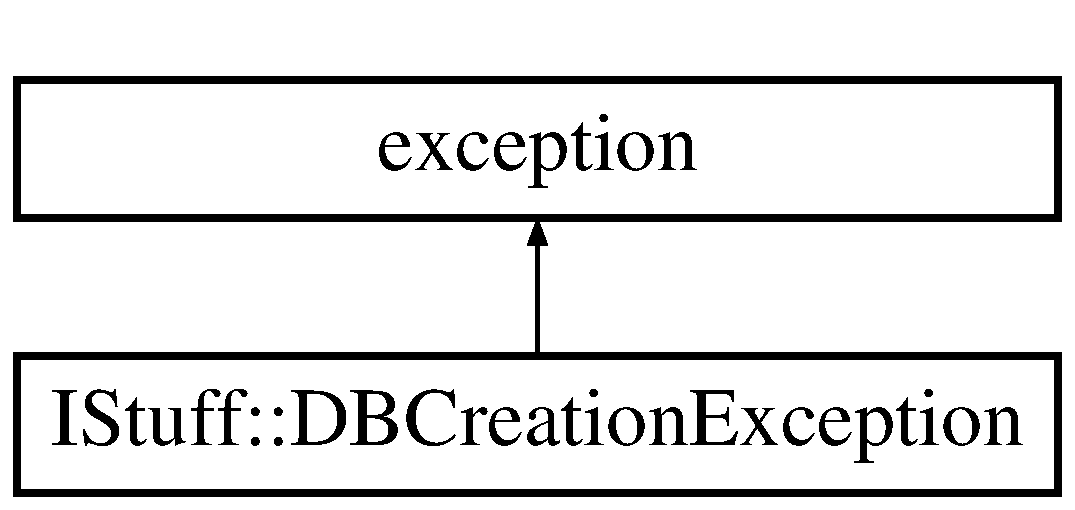
\includegraphics[height=2.000000cm]{class_i_stuff_1_1_d_b_creation_exception}
\end{center}
\end{figure}
\subsection*{Public Member Functions}
\begin{DoxyCompactItemize}
\item 
virtual const char $\ast$ \hyperlink{class_i_stuff_1_1_d_b_creation_exception_ab3d2214cbcbc3d495483bd2bce8f4d81}{what} () const   throw ()
\end{DoxyCompactItemize}


\subsection{Detailed Description}


Definition at line 75 of file database.\-h.



\subsection{Member Function Documentation}
\hypertarget{class_i_stuff_1_1_d_b_creation_exception_ab3d2214cbcbc3d495483bd2bce8f4d81}{\index{I\-Stuff\-::\-D\-B\-Creation\-Exception@{I\-Stuff\-::\-D\-B\-Creation\-Exception}!what@{what}}
\index{what@{what}!IStuff::DBCreationException@{I\-Stuff\-::\-D\-B\-Creation\-Exception}}
\subsubsection[{what}]{\setlength{\rightskip}{0pt plus 5cm}virtual const char$\ast$ I\-Stuff\-::\-D\-B\-Creation\-Exception\-::what (
\begin{DoxyParamCaption}
{}
\end{DoxyParamCaption}
) const throw  ) \hspace{0.3cm}{\ttfamily [inline]}, {\ttfamily [virtual]}}}\label{class_i_stuff_1_1_d_b_creation_exception_ab3d2214cbcbc3d495483bd2bce8f4d81}


Definition at line 76 of file database.\-h.



The documentation for this class was generated from the following file\-:\begin{DoxyCompactItemize}
\item 
src/\-I\-Stuff/\hyperlink{database_8h}{database.\-h}\end{DoxyCompactItemize}

\hypertarget{class_i_stuff_1_1_d_b_loading_exception}{\section{I\-Stuff\-:\-:D\-B\-Loading\-Exception Class Reference}
\label{class_i_stuff_1_1_d_b_loading_exception}\index{I\-Stuff\-::\-D\-B\-Loading\-Exception@{I\-Stuff\-::\-D\-B\-Loading\-Exception}}
}


{\ttfamily \#include $<$database.\-h$>$}

Inheritance diagram for I\-Stuff\-:\-:D\-B\-Loading\-Exception\-:\begin{figure}[H]
\begin{center}
\leavevmode
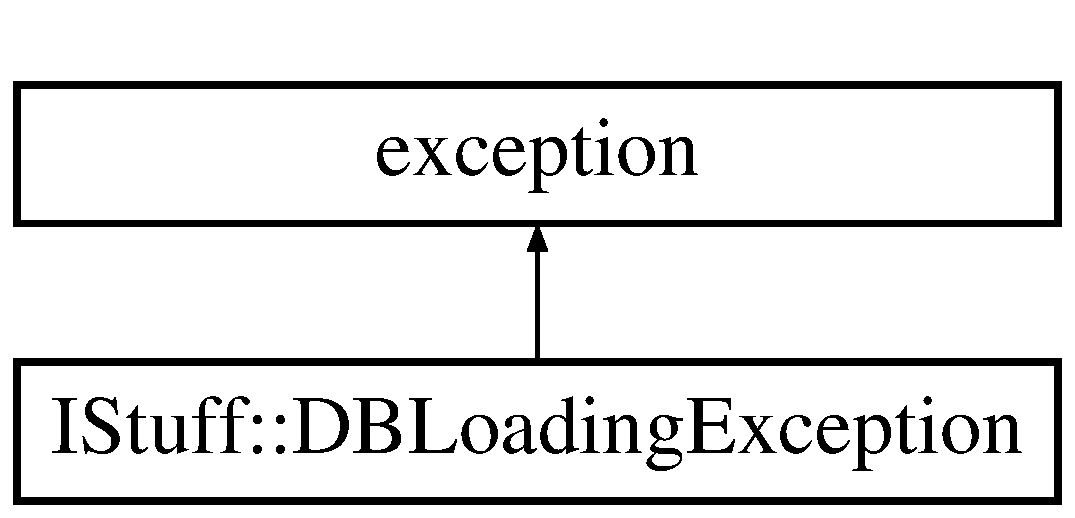
\includegraphics[height=2.000000cm]{class_i_stuff_1_1_d_b_loading_exception}
\end{center}
\end{figure}
\subsection*{Public Member Functions}
\begin{DoxyCompactItemize}
\item 
virtual const char $\ast$ \hyperlink{class_i_stuff_1_1_d_b_loading_exception_aadb5bf6ac0fa6b4f84433261003e5e64}{what} () const   throw ()
\end{DoxyCompactItemize}


\subsection{Detailed Description}


Definition at line 76 of file database.\-h.



\subsection{Member Function Documentation}
\hypertarget{class_i_stuff_1_1_d_b_loading_exception_aadb5bf6ac0fa6b4f84433261003e5e64}{\index{I\-Stuff\-::\-D\-B\-Loading\-Exception@{I\-Stuff\-::\-D\-B\-Loading\-Exception}!what@{what}}
\index{what@{what}!IStuff::DBLoadingException@{I\-Stuff\-::\-D\-B\-Loading\-Exception}}
\subsubsection[{what}]{\setlength{\rightskip}{0pt plus 5cm}virtual const char$\ast$ I\-Stuff\-::\-D\-B\-Loading\-Exception\-::what (
\begin{DoxyParamCaption}
{}
\end{DoxyParamCaption}
) const throw  ) \hspace{0.3cm}{\ttfamily [inline]}, {\ttfamily [virtual]}}}\label{class_i_stuff_1_1_d_b_loading_exception_aadb5bf6ac0fa6b4f84433261003e5e64}


Definition at line 77 of file database.\-h.



The documentation for this class was generated from the following file\-:\begin{DoxyCompactItemize}
\item 
src/\-I\-Stuff/\hyperlink{database_8h}{database.\-h}\end{DoxyCompactItemize}

\hypertarget{class_i_stuff_1_1_d_b_saving_exception}{\section{I\-Stuff\-:\-:D\-B\-Saving\-Exception Class Reference}
\label{class_i_stuff_1_1_d_b_saving_exception}\index{I\-Stuff\-::\-D\-B\-Saving\-Exception@{I\-Stuff\-::\-D\-B\-Saving\-Exception}}
}


{\ttfamily \#include $<$database.\-h$>$}

Inheritance diagram for I\-Stuff\-:\-:D\-B\-Saving\-Exception\-:\begin{figure}[H]
\begin{center}
\leavevmode
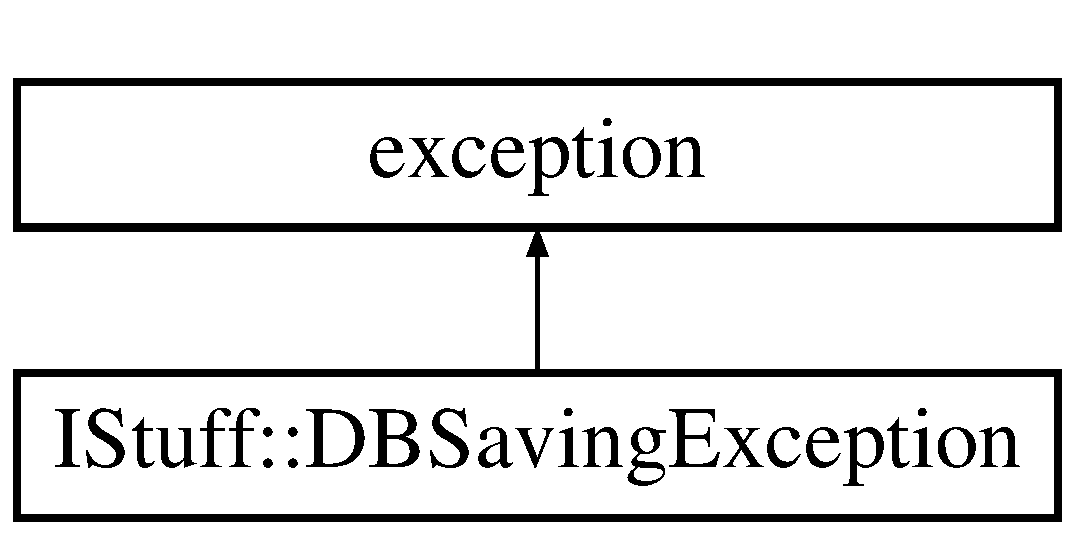
\includegraphics[height=2.000000cm]{class_i_stuff_1_1_d_b_saving_exception}
\end{center}
\end{figure}
\subsection*{Public Member Functions}
\begin{DoxyCompactItemize}
\item 
virtual const char $\ast$ \hyperlink{class_i_stuff_1_1_d_b_saving_exception_a1b55277b5e63b468f1e717db118101d4}{what} () const   throw ()
\end{DoxyCompactItemize}


\subsection{Detailed Description}


Definition at line 87 of file database.\-h.



\subsection{Member Function Documentation}
\hypertarget{class_i_stuff_1_1_d_b_saving_exception_a1b55277b5e63b468f1e717db118101d4}{\index{I\-Stuff\-::\-D\-B\-Saving\-Exception@{I\-Stuff\-::\-D\-B\-Saving\-Exception}!what@{what}}
\index{what@{what}!IStuff::DBSavingException@{I\-Stuff\-::\-D\-B\-Saving\-Exception}}
\subsubsection[{what}]{\setlength{\rightskip}{0pt plus 5cm}virtual const char$\ast$ I\-Stuff\-::\-D\-B\-Saving\-Exception\-::what (
\begin{DoxyParamCaption}
{}
\end{DoxyParamCaption}
) const throw  ) \hspace{0.3cm}{\ttfamily [inline]}, {\ttfamily [virtual]}}}\label{class_i_stuff_1_1_d_b_saving_exception_a1b55277b5e63b468f1e717db118101d4}


Definition at line 88 of file database.\-h.



The documentation for this class was generated from the following file\-:\begin{DoxyCompactItemize}
\item 
src/\-I\-Stuff/\hyperlink{database_8h}{database.\-h}\end{DoxyCompactItemize}

\hypertarget{class_i_stuff_1_1_fakable_queue}{\section{I\-Stuff\-:\-:Fakable\-Queue Class Reference}
\label{class_i_stuff_1_1_fakable_queue}\index{I\-Stuff\-::\-Fakable\-Queue@{I\-Stuff\-::\-Fakable\-Queue}}
}


Class used to manage a synchronized double queue.  




{\ttfamily \#include $<$fakable\-\_\-queue.\-h$>$}

\subsection*{Public Member Functions}
\begin{DoxyCompactItemize}
\item 
\hyperlink{class_i_stuff_1_1_fakable_queue_a22906efd165f0becf24bc4056b966fb6}{Fakable\-Queue} ()
\begin{DoxyCompactList}\small\item\em Constructor of this class. \end{DoxyCompactList}\item 
virtual \hyperlink{class_i_stuff_1_1_fakable_queue_a9675cd13bcaa59d614d47127c0c21d93}{$\sim$\-Fakable\-Queue} ()
\item 
void \hyperlink{class_i_stuff_1_1_fakable_queue_a2d615a3f5fb3bbe26bd99694bd1a2378}{enqueue} (cv\-::\-Mat)
\begin{DoxyCompactList}\small\item\em Adds a frame to the queue. \end{DoxyCompactList}\item 
void \hyperlink{class_i_stuff_1_1_fakable_queue_acb05a50ab738a9df2cccf7b697c199ca}{start} (cv\-::\-Mat)
\begin{DoxyCompactList}\small\item\em Starts the queue, enabiling the enqueuement. \end{DoxyCompactList}\item 
void \hyperlink{class_i_stuff_1_1_fakable_queue_a5f103ad2380d4aaf9c38c8853c3c97a9}{discard} ()
\begin{DoxyCompactList}\small\item\em Replaces the 'real' queue with the 'saved' one. \end{DoxyCompactList}\item 
cv\-::\-Mat \hyperlink{class_i_stuff_1_1_fakable_queue_a45d9c3549edcd23c87d70142db01df05}{dequeue} ()
\begin{DoxyCompactList}\small\item\em Returns and removes a frame from the 'real' queue. \end{DoxyCompactList}\item 
cv\-::\-Mat \hyperlink{class_i_stuff_1_1_fakable_queue_aea66bd432f26ee1322387dc5589b721d}{get\-Starter} ()
\begin{DoxyCompactList}\small\item\em Returns the frame that started the queue. \end{DoxyCompactList}\end{DoxyCompactItemize}
\subsection*{Private Attributes}
\begin{DoxyCompactItemize}
\item 
std\-::queue$<$ cv\-::\-Mat $>$ \hyperlink{class_i_stuff_1_1_fakable_queue_a572a03879f073d8fa1babbfbf4b9d573}{real\-\_\-queue}
\item 
std\-::queue$<$ cv\-::\-Mat $>$ \hyperlink{class_i_stuff_1_1_fakable_queue_a4204d286617b6b3e9c1732946e06d0ad}{saved\-\_\-queue}
\item 
boost\-::mutex \hyperlink{class_i_stuff_1_1_fakable_queue_a463ced47c344cac9858ddb9c3a2a5fc6}{queue\-\_\-mutex}
\end{DoxyCompactItemize}
\subsection*{Static Private Attributes}
\begin{DoxyCompactItemize}
\item 
static const char \hyperlink{class_i_stuff_1_1_fakable_queue_a0934f12df566975c8811084f54aa8247}{T\-A\-G} \mbox{[}$\,$\mbox{]} = \char`\"{}Fkq\char`\"{}
\end{DoxyCompactItemize}


\subsection{Detailed Description}
Class used to manage a synchronized double queue. 

This class is used by \hyperlink{class_i_stuff_1_1_tracker}{I\-Stuff\-::\-Tracker} and it allows to address problems caused by alternated recognizations\-:\par
 This queue manages two queues\-: one \char`\"{}real\char`\"{}, used normally, from where frames are enqueued and dequeued and one \char`\"{}fake\char`\"{}, or \char`\"{}saved\char`\"{}, used to store the frames regarding only the last recognization, where frames are just enqueued and which is substituted to the real queue when the last recognization ends. \begin{DoxyAuthor}{Author}
Maurizio Zucchelli 
\end{DoxyAuthor}
\begin{DoxyVersion}{Version}
0.\-1.\-2 
\end{DoxyVersion}
\begin{DoxyDate}{Date}
2013-\/07-\/18 
\end{DoxyDate}


Definition at line 23 of file fakable\-\_\-queue.\-h.



\subsection{Constructor \& Destructor Documentation}
\hypertarget{class_i_stuff_1_1_fakable_queue_a22906efd165f0becf24bc4056b966fb6}{\index{I\-Stuff\-::\-Fakable\-Queue@{I\-Stuff\-::\-Fakable\-Queue}!Fakable\-Queue@{Fakable\-Queue}}
\index{Fakable\-Queue@{Fakable\-Queue}!IStuff::FakableQueue@{I\-Stuff\-::\-Fakable\-Queue}}
\subsubsection[{Fakable\-Queue}]{\setlength{\rightskip}{0pt plus 5cm}Fakable\-Queue\-::\-Fakable\-Queue (
\begin{DoxyParamCaption}
{}
\end{DoxyParamCaption}
)}}\label{class_i_stuff_1_1_fakable_queue_a22906efd165f0becf24bc4056b966fb6}


Constructor of this class. 



Definition at line 30 of file fakable\-\_\-queue.\-cpp.

\hypertarget{class_i_stuff_1_1_fakable_queue_a9675cd13bcaa59d614d47127c0c21d93}{\index{I\-Stuff\-::\-Fakable\-Queue@{I\-Stuff\-::\-Fakable\-Queue}!$\sim$\-Fakable\-Queue@{$\sim$\-Fakable\-Queue}}
\index{$\sim$\-Fakable\-Queue@{$\sim$\-Fakable\-Queue}!IStuff::FakableQueue@{I\-Stuff\-::\-Fakable\-Queue}}
\subsubsection[{$\sim$\-Fakable\-Queue}]{\setlength{\rightskip}{0pt plus 5cm}Fakable\-Queue\-::$\sim$\-Fakable\-Queue (
\begin{DoxyParamCaption}
{}
\end{DoxyParamCaption}
)\hspace{0.3cm}{\ttfamily [virtual]}}}\label{class_i_stuff_1_1_fakable_queue_a9675cd13bcaa59d614d47127c0c21d93}


Definition at line 33 of file fakable\-\_\-queue.\-cpp.



\subsection{Member Function Documentation}
\hypertarget{class_i_stuff_1_1_fakable_queue_a45d9c3549edcd23c87d70142db01df05}{\index{I\-Stuff\-::\-Fakable\-Queue@{I\-Stuff\-::\-Fakable\-Queue}!dequeue@{dequeue}}
\index{dequeue@{dequeue}!IStuff::FakableQueue@{I\-Stuff\-::\-Fakable\-Queue}}
\subsubsection[{dequeue}]{\setlength{\rightskip}{0pt plus 5cm}Mat Fakable\-Queue\-::dequeue (
\begin{DoxyParamCaption}
{}
\end{DoxyParamCaption}
)}}\label{class_i_stuff_1_1_fakable_queue_a45d9c3549edcd23c87d70142db01df05}


Returns and removes a frame from the 'real' queue. 


\begin{DoxyExceptions}{Exceptions}
{\em out\-\_\-of\-\_\-range} & If the queue is empty.\\
\hline
\end{DoxyExceptions}
\begin{DoxyReturn}{Returns}
The frame in front of the 'real' queue. 
\end{DoxyReturn}


Definition at line 103 of file fakable\-\_\-queue.\-cpp.

\hypertarget{class_i_stuff_1_1_fakable_queue_a5f103ad2380d4aaf9c38c8853c3c97a9}{\index{I\-Stuff\-::\-Fakable\-Queue@{I\-Stuff\-::\-Fakable\-Queue}!discard@{discard}}
\index{discard@{discard}!IStuff::FakableQueue@{I\-Stuff\-::\-Fakable\-Queue}}
\subsubsection[{discard}]{\setlength{\rightskip}{0pt plus 5cm}void Fakable\-Queue\-::discard (
\begin{DoxyParamCaption}
{}
\end{DoxyParamCaption}
)}}\label{class_i_stuff_1_1_fakable_queue_a5f103ad2380d4aaf9c38c8853c3c97a9}


Replaces the 'real' queue with the 'saved' one. 

\begin{DoxyRefDesc}{Todo}
\item[\hyperlink{todo__todo000001}{Todo}]Find a more explicative name. \end{DoxyRefDesc}


Definition at line 85 of file fakable\-\_\-queue.\-cpp.

\hypertarget{class_i_stuff_1_1_fakable_queue_a2d615a3f5fb3bbe26bd99694bd1a2378}{\index{I\-Stuff\-::\-Fakable\-Queue@{I\-Stuff\-::\-Fakable\-Queue}!enqueue@{enqueue}}
\index{enqueue@{enqueue}!IStuff::FakableQueue@{I\-Stuff\-::\-Fakable\-Queue}}
\subsubsection[{enqueue}]{\setlength{\rightskip}{0pt plus 5cm}void Fakable\-Queue\-::enqueue (
\begin{DoxyParamCaption}
\item[{cv\-::\-Mat}]{}
\end{DoxyParamCaption}
)}}\label{class_i_stuff_1_1_fakable_queue_a2d615a3f5fb3bbe26bd99694bd1a2378}


Adds a frame to the queue. 

If the queue has been started, the frame is added to both the 'real' and the 'saved' queue; otherwise, nothing happens.


\begin{DoxyParams}[1]{Parameters}
\mbox{\tt in}  & {\em frame} & The frame to be inserted. \\
\hline
\end{DoxyParams}


Definition at line 45 of file fakable\-\_\-queue.\-cpp.

\hypertarget{class_i_stuff_1_1_fakable_queue_aea66bd432f26ee1322387dc5589b721d}{\index{I\-Stuff\-::\-Fakable\-Queue@{I\-Stuff\-::\-Fakable\-Queue}!get\-Starter@{get\-Starter}}
\index{get\-Starter@{get\-Starter}!IStuff::FakableQueue@{I\-Stuff\-::\-Fakable\-Queue}}
\subsubsection[{get\-Starter}]{\setlength{\rightskip}{0pt plus 5cm}Mat Fakable\-Queue\-::get\-Starter (
\begin{DoxyParamCaption}
{}
\end{DoxyParamCaption}
)}}\label{class_i_stuff_1_1_fakable_queue_aea66bd432f26ee1322387dc5589b721d}


Returns the frame that started the queue. 

\begin{DoxyReturn}{Returns}
The frame that started the queue. 
\end{DoxyReturn}


Definition at line 126 of file fakable\-\_\-queue.\-cpp.

\hypertarget{class_i_stuff_1_1_fakable_queue_acb05a50ab738a9df2cccf7b697c199ca}{\index{I\-Stuff\-::\-Fakable\-Queue@{I\-Stuff\-::\-Fakable\-Queue}!start@{start}}
\index{start@{start}!IStuff::FakableQueue@{I\-Stuff\-::\-Fakable\-Queue}}
\subsubsection[{start}]{\setlength{\rightskip}{0pt plus 5cm}void Fakable\-Queue\-::start (
\begin{DoxyParamCaption}
\item[{cv\-::\-Mat}]{}
\end{DoxyParamCaption}
)}}\label{class_i_stuff_1_1_fakable_queue_acb05a50ab738a9df2cccf7b697c199ca}


Starts the queue, enabiling the enqueuement. 

This operation resets the 'saved' queue and then performs an enqueue with the given frame.


\begin{DoxyParams}[1]{Parameters}
\mbox{\tt in}  & {\em frame} & The frame starter of the queue. \\
\hline
\end{DoxyParams}


Definition at line 68 of file fakable\-\_\-queue.\-cpp.



\subsection{Member Data Documentation}
\hypertarget{class_i_stuff_1_1_fakable_queue_a463ced47c344cac9858ddb9c3a2a5fc6}{\index{I\-Stuff\-::\-Fakable\-Queue@{I\-Stuff\-::\-Fakable\-Queue}!queue\-\_\-mutex@{queue\-\_\-mutex}}
\index{queue\-\_\-mutex@{queue\-\_\-mutex}!IStuff::FakableQueue@{I\-Stuff\-::\-Fakable\-Queue}}
\subsubsection[{queue\-\_\-mutex}]{\setlength{\rightskip}{0pt plus 5cm}boost\-::mutex I\-Stuff\-::\-Fakable\-Queue\-::queue\-\_\-mutex\hspace{0.3cm}{\ttfamily [private]}}}\label{class_i_stuff_1_1_fakable_queue_a463ced47c344cac9858ddb9c3a2a5fc6}


Definition at line 31 of file fakable\-\_\-queue.\-h.

\hypertarget{class_i_stuff_1_1_fakable_queue_a572a03879f073d8fa1babbfbf4b9d573}{\index{I\-Stuff\-::\-Fakable\-Queue@{I\-Stuff\-::\-Fakable\-Queue}!real\-\_\-queue@{real\-\_\-queue}}
\index{real\-\_\-queue@{real\-\_\-queue}!IStuff::FakableQueue@{I\-Stuff\-::\-Fakable\-Queue}}
\subsubsection[{real\-\_\-queue}]{\setlength{\rightskip}{0pt plus 5cm}std\-::queue$<$cv\-::\-Mat$>$ I\-Stuff\-::\-Fakable\-Queue\-::real\-\_\-queue\hspace{0.3cm}{\ttfamily [private]}}}\label{class_i_stuff_1_1_fakable_queue_a572a03879f073d8fa1babbfbf4b9d573}


Definition at line 29 of file fakable\-\_\-queue.\-h.

\hypertarget{class_i_stuff_1_1_fakable_queue_a4204d286617b6b3e9c1732946e06d0ad}{\index{I\-Stuff\-::\-Fakable\-Queue@{I\-Stuff\-::\-Fakable\-Queue}!saved\-\_\-queue@{saved\-\_\-queue}}
\index{saved\-\_\-queue@{saved\-\_\-queue}!IStuff::FakableQueue@{I\-Stuff\-::\-Fakable\-Queue}}
\subsubsection[{saved\-\_\-queue}]{\setlength{\rightskip}{0pt plus 5cm}std\-::queue$<$cv\-::\-Mat$>$ I\-Stuff\-::\-Fakable\-Queue\-::saved\-\_\-queue\hspace{0.3cm}{\ttfamily [private]}}}\label{class_i_stuff_1_1_fakable_queue_a4204d286617b6b3e9c1732946e06d0ad}


Definition at line 29 of file fakable\-\_\-queue.\-h.

\hypertarget{class_i_stuff_1_1_fakable_queue_a0934f12df566975c8811084f54aa8247}{\index{I\-Stuff\-::\-Fakable\-Queue@{I\-Stuff\-::\-Fakable\-Queue}!T\-A\-G@{T\-A\-G}}
\index{T\-A\-G@{T\-A\-G}!IStuff::FakableQueue@{I\-Stuff\-::\-Fakable\-Queue}}
\subsubsection[{T\-A\-G}]{\setlength{\rightskip}{0pt plus 5cm}const char Fakable\-Queue\-::\-T\-A\-G = \char`\"{}Fkq\char`\"{}\hspace{0.3cm}{\ttfamily [static]}, {\ttfamily [private]}}}\label{class_i_stuff_1_1_fakable_queue_a0934f12df566975c8811084f54aa8247}


Definition at line 27 of file fakable\-\_\-queue.\-h.



The documentation for this class was generated from the following files\-:\begin{DoxyCompactItemize}
\item 
src/\-I\-Stuff/\hyperlink{fakable__queue_8h}{fakable\-\_\-queue.\-h}\item 
src/\-I\-Stuff/\hyperlink{fakable__queue_8cpp}{fakable\-\_\-queue.\-cpp}\end{DoxyCompactItemize}

\hypertarget{struct_i_stuff_1_1_label}{\section{I\-Stuff\-:\-:Label Struct Reference}
\label{struct_i_stuff_1_1_label}\index{I\-Stuff\-::\-Label@{I\-Stuff\-::\-Label}}
}


\hyperlink{struct_i_stuff_1_1_label}{Label} relative to a view of an \hyperlink{class_i_stuff_1_1_object}{Object}.  




{\ttfamily \#include $<$object.\-h$>$}

\subsection*{Public Member Functions}
\begin{DoxyCompactItemize}
\item 
\hyperlink{struct_i_stuff_1_1_label_aac1f21d615fb8b65f18c7ad76b63e6cf}{Label} (std\-::string \-\_\-name, cv\-::\-Point2f \-\_\-position, cv\-::\-Scalar \-\_\-color)
\item 
bool \hyperlink{struct_i_stuff_1_1_label_af37f54284d7c8f2232b1273bf6be1e96}{operator==} (const \hyperlink{struct_i_stuff_1_1_label}{Label} \&other) const 
\end{DoxyCompactItemize}
\subsection*{Public Attributes}
\begin{DoxyCompactItemize}
\item 
std\-::string \hyperlink{struct_i_stuff_1_1_label_a11026b588c7a66f59bf233529c9aa6ed}{name}
\item 
cv\-::\-Point2f \hyperlink{struct_i_stuff_1_1_label_a06b344b0151f8c836e89d885a2e96975}{position}
\item 
cv\-::\-Scalar \hyperlink{struct_i_stuff_1_1_label_aaa492eddf40936c251bcd5b920e9d696}{color}
\end{DoxyCompactItemize}


\subsection{Detailed Description}
\hyperlink{struct_i_stuff_1_1_label}{Label} relative to a view of an \hyperlink{class_i_stuff_1_1_object}{Object}. 

Definition at line 26 of file object.\-h.



\subsection{Constructor \& Destructor Documentation}
\hypertarget{struct_i_stuff_1_1_label_aac1f21d615fb8b65f18c7ad76b63e6cf}{\index{I\-Stuff\-::\-Label@{I\-Stuff\-::\-Label}!Label@{Label}}
\index{Label@{Label}!IStuff::Label@{I\-Stuff\-::\-Label}}
\subsubsection[{Label}]{\setlength{\rightskip}{0pt plus 5cm}I\-Stuff\-::\-Label\-::\-Label (
\begin{DoxyParamCaption}
\item[{std\-::string}]{\-\_\-name, }
\item[{cv\-::\-Point2f}]{\-\_\-position, }
\item[{cv\-::\-Scalar}]{\-\_\-color}
\end{DoxyParamCaption}
)\hspace{0.3cm}{\ttfamily [inline]}}}\label{struct_i_stuff_1_1_label_aac1f21d615fb8b65f18c7ad76b63e6cf}


Definition at line 31 of file object.\-h.



\subsection{Member Function Documentation}
\hypertarget{struct_i_stuff_1_1_label_af37f54284d7c8f2232b1273bf6be1e96}{\index{I\-Stuff\-::\-Label@{I\-Stuff\-::\-Label}!operator==@{operator==}}
\index{operator==@{operator==}!IStuff::Label@{I\-Stuff\-::\-Label}}
\subsubsection[{operator==}]{\setlength{\rightskip}{0pt plus 5cm}bool I\-Stuff\-::\-Label\-::operator== (
\begin{DoxyParamCaption}
\item[{const {\bf Label} \&}]{other}
\end{DoxyParamCaption}
) const\hspace{0.3cm}{\ttfamily [inline]}}}\label{struct_i_stuff_1_1_label_af37f54284d7c8f2232b1273bf6be1e96}


Definition at line 35 of file object.\-h.



\subsection{Member Data Documentation}
\hypertarget{struct_i_stuff_1_1_label_aaa492eddf40936c251bcd5b920e9d696}{\index{I\-Stuff\-::\-Label@{I\-Stuff\-::\-Label}!color@{color}}
\index{color@{color}!IStuff::Label@{I\-Stuff\-::\-Label}}
\subsubsection[{color}]{\setlength{\rightskip}{0pt plus 5cm}cv\-::\-Scalar I\-Stuff\-::\-Label\-::color}}\label{struct_i_stuff_1_1_label_aaa492eddf40936c251bcd5b920e9d696}


Definition at line 29 of file object.\-h.

\hypertarget{struct_i_stuff_1_1_label_a11026b588c7a66f59bf233529c9aa6ed}{\index{I\-Stuff\-::\-Label@{I\-Stuff\-::\-Label}!name@{name}}
\index{name@{name}!IStuff::Label@{I\-Stuff\-::\-Label}}
\subsubsection[{name}]{\setlength{\rightskip}{0pt plus 5cm}std\-::string I\-Stuff\-::\-Label\-::name}}\label{struct_i_stuff_1_1_label_a11026b588c7a66f59bf233529c9aa6ed}


Definition at line 27 of file object.\-h.

\hypertarget{struct_i_stuff_1_1_label_a06b344b0151f8c836e89d885a2e96975}{\index{I\-Stuff\-::\-Label@{I\-Stuff\-::\-Label}!position@{position}}
\index{position@{position}!IStuff::Label@{I\-Stuff\-::\-Label}}
\subsubsection[{position}]{\setlength{\rightskip}{0pt plus 5cm}cv\-::\-Point2f I\-Stuff\-::\-Label\-::position}}\label{struct_i_stuff_1_1_label_a06b344b0151f8c836e89d885a2e96975}


Definition at line 28 of file object.\-h.



The documentation for this struct was generated from the following file\-:\begin{DoxyCompactItemize}
\item 
src/\-I\-Stuff/\hyperlink{object_8h}{object.\-h}\end{DoxyCompactItemize}

\hypertarget{class_i_stuff_1_1_manager}{\section{I\-Stuff\-:\-:Manager Class Reference}
\label{class_i_stuff_1_1_manager}\index{I\-Stuff\-::\-Manager@{I\-Stuff\-::\-Manager}}
}


Class to manage the joint 3\-D \hyperlink{class_i_stuff_1_1_object}{Object} recognition and tracking.  




{\ttfamily \#include $<$manager.\-h$>$}

\subsection*{Public Member Functions}
\begin{DoxyCompactItemize}
\item 
\hyperlink{class_i_stuff_1_1_manager_a1658ff9f18e38ccd9cb8b0b371b9c20b}{Manager} ()
\begin{DoxyCompactList}\small\item\em Constructs the class. \end{DoxyCompactList}\item 
virtual \hyperlink{class_i_stuff_1_1_manager_a322cad25d7007438b3a043ad02253d29}{$\sim$\-Manager} ()
\item 
void \hyperlink{class_i_stuff_1_1_manager_aa91ba11affc3ec961acaf81fc5c5e62d}{set\-Database} (\hyperlink{class_i_stuff_1_1_database}{Database} $\ast$)
\begin{DoxyCompactList}\small\item\em Changes the \hyperlink{class_i_stuff_1_1_database}{I\-Stuff\-::\-Database} used to identify the \hyperlink{class_i_stuff_1_1_object}{I\-Stuff\-::\-Object}. \end{DoxyCompactList}\item 
\hyperlink{class_i_stuff_1_1_object}{Object} \hyperlink{class_i_stuff_1_1_manager_a80d15a0a83976f63c357f65b20387e02}{get\-Object} ()
\begin{DoxyCompactList}\small\item\em Returns the current description of the \hyperlink{class_i_stuff_1_1_object}{I\-Stuff\-::\-Object}. \end{DoxyCompactList}\item 
void \hyperlink{class_i_stuff_1_1_manager_a47f17fa372382713bcc0f37aae006745}{elaborate\-Frame} (cv\-::\-Mat)
\begin{DoxyCompactList}\small\item\em Elaborates a frame, searching for the \hyperlink{class_i_stuff_1_1_object}{I\-Stuff\-::\-Object}. \end{DoxyCompactList}\item 
cv\-::\-Mat \hyperlink{class_i_stuff_1_1_manager_a5cc4e8151aa21b873786eb8c0742c3d5}{paint\-Object} (cv\-::\-Mat)
\begin{DoxyCompactList}\small\item\em Paints the various masks of the \hyperlink{class_i_stuff_1_1_object}{I\-Stuff\-::\-Object} on the frame. \end{DoxyCompactList}\item 
void \hyperlink{class_i_stuff_1_1_manager_adaef1575710c20ad769c23bb55d2144c}{send\-Message} (int, void $\ast$, void $\ast$=N\-U\-L\-L)
\begin{DoxyCompactList}\small\item\em Method to send messages to this \hyperlink{class_i_stuff_1_1_manager}{I\-Stuff\-::\-Manager}. \end{DoxyCompactList}\end{DoxyCompactItemize}
\subsection*{Static Public Attributes}
\begin{DoxyCompactItemize}
\item 
static const int \hyperlink{class_i_stuff_1_1_manager_af7f9a2cc3c53b7cf351a12f179230da7}{M\-S\-G\-\_\-\-R\-E\-C\-O\-G\-N\-I\-T\-I\-O\-N\-\_\-\-S\-T\-A\-R\-T} = 1
\item 
static const int \hyperlink{class_i_stuff_1_1_manager_a4c465ff50b8eddde0e5fd8b4d3e37bbc}{M\-S\-G\-\_\-\-R\-E\-C\-O\-G\-N\-I\-T\-I\-O\-N\-\_\-\-E\-N\-D} = 2
\item 
static const int \hyperlink{class_i_stuff_1_1_manager_a46dc3e50421b203bab7941bcc6e29604}{M\-S\-G\-\_\-\-T\-R\-A\-C\-K\-I\-N\-G\-\_\-\-S\-T\-A\-R\-T} = 3
\item 
static const int \hyperlink{class_i_stuff_1_1_manager_a841fb5e820b9aa16aa8d7862362fa50b}{M\-S\-G\-\_\-\-T\-R\-A\-C\-K\-I\-N\-G\-\_\-\-E\-N\-D} = 4
\end{DoxyCompactItemize}
\subsection*{Private Member Functions}
\begin{DoxyCompactItemize}
\item 
void \hyperlink{class_i_stuff_1_1_manager_a3cc212bd05afe4bdffada9dd35994c61}{set\-Object} (const \hyperlink{class_i_stuff_1_1_object}{Object})
\begin{DoxyCompactList}\small\item\em Sets the \hyperlink{class_i_stuff_1_1_object}{I\-Stuff\-::\-Object} of this \hyperlink{class_i_stuff_1_1_manager}{I\-Stuff\-::\-Manager}. \end{DoxyCompactList}\end{DoxyCompactItemize}
\subsection*{Private Attributes}
\begin{DoxyCompactItemize}
\item 
int \hyperlink{class_i_stuff_1_1_manager_a3cacb02ece1a4938e7754ad553c91a74}{frames\-\_\-tracked\-\_\-count}
\begin{DoxyCompactList}\small\item\em When this reaches R\-E\-C\-O\-G\-N\-I\-T\-I\-O\-N\-\_\-\-P\-E\-R\-I\-O\-D, a new recognition is done. \end{DoxyCompactList}\item 
boost\-::shared\-\_\-mutex \hyperlink{class_i_stuff_1_1_manager_a9b4234320a01a049bc10f9f13d612fc4}{object\-\_\-update}
\item 
\hyperlink{class_i_stuff_1_1_object}{Object} \hyperlink{class_i_stuff_1_1_manager_a9b898107c919a3ba73f60278c9c05742}{actual\-\_\-object}
\item 
\hyperlink{class_i_stuff_1_1_recognizer}{Recognizer} \hyperlink{class_i_stuff_1_1_manager_ac039aa2e611b04595e4ff69d3534b4cc}{recognizer}
\item 
\hyperlink{class_i_stuff_1_1_tracker}{Tracker} \hyperlink{class_i_stuff_1_1_manager_a3d313f62a1cfe606098fdcb6f1c748ee}{tracker}
\end{DoxyCompactItemize}
\subsection*{Static Private Attributes}
\begin{DoxyCompactItemize}
\item 
static const char \hyperlink{class_i_stuff_1_1_manager_a0228682f317a86ce7057b86e9d229ac6}{T\-A\-G} \mbox{[}$\,$\mbox{]} = \char`\"{}Mng\char`\"{}
\item 
static const int \hyperlink{class_i_stuff_1_1_manager_a58f0beb39eea21e78a8983e5954065c3}{R\-E\-C\-O\-G\-N\-I\-T\-I\-O\-N\-\_\-\-P\-E\-R\-I\-O\-D} = 50
\end{DoxyCompactItemize}


\subsection{Detailed Description}
Class to manage the joint 3\-D \hyperlink{class_i_stuff_1_1_object}{Object} recognition and tracking. 

\begin{DoxyAuthor}{Author}
Maurizio Zucchelli 
\end{DoxyAuthor}
\begin{DoxyVersion}{Version}
0.\-3.\-0 
\end{DoxyVersion}
\begin{DoxyDate}{Date}
2013-\/07-\/16 
\end{DoxyDate}


Definition at line 28 of file manager.\-h.



\subsection{Constructor \& Destructor Documentation}
\hypertarget{class_i_stuff_1_1_manager_a1658ff9f18e38ccd9cb8b0b371b9c20b}{\index{I\-Stuff\-::\-Manager@{I\-Stuff\-::\-Manager}!Manager@{Manager}}
\index{Manager@{Manager}!IStuff::Manager@{I\-Stuff\-::\-Manager}}
\subsubsection[{Manager}]{\setlength{\rightskip}{0pt plus 5cm}Manager\-::\-Manager (
\begin{DoxyParamCaption}
{}
\end{DoxyParamCaption}
)}}\label{class_i_stuff_1_1_manager_a1658ff9f18e38ccd9cb8b0b371b9c20b}


Constructs the class. 



Definition at line 24 of file manager.\-cpp.

\hypertarget{class_i_stuff_1_1_manager_a322cad25d7007438b3a043ad02253d29}{\index{I\-Stuff\-::\-Manager@{I\-Stuff\-::\-Manager}!$\sim$\-Manager@{$\sim$\-Manager}}
\index{$\sim$\-Manager@{$\sim$\-Manager}!IStuff::Manager@{I\-Stuff\-::\-Manager}}
\subsubsection[{$\sim$\-Manager}]{\setlength{\rightskip}{0pt plus 5cm}Manager\-::$\sim$\-Manager (
\begin{DoxyParamCaption}
{}
\end{DoxyParamCaption}
)\hspace{0.3cm}{\ttfamily [virtual]}}}\label{class_i_stuff_1_1_manager_a322cad25d7007438b3a043ad02253d29}


Definition at line 29 of file manager.\-cpp.



\subsection{Member Function Documentation}
\hypertarget{class_i_stuff_1_1_manager_a47f17fa372382713bcc0f37aae006745}{\index{I\-Stuff\-::\-Manager@{I\-Stuff\-::\-Manager}!elaborate\-Frame@{elaborate\-Frame}}
\index{elaborate\-Frame@{elaborate\-Frame}!IStuff::Manager@{I\-Stuff\-::\-Manager}}
\subsubsection[{elaborate\-Frame}]{\setlength{\rightskip}{0pt plus 5cm}void Manager\-::elaborate\-Frame (
\begin{DoxyParamCaption}
\item[{cv\-::\-Mat}]{}
\end{DoxyParamCaption}
)}}\label{class_i_stuff_1_1_manager_a47f17fa372382713bcc0f37aae006745}


Elaborates a frame, searching for the \hyperlink{class_i_stuff_1_1_object}{I\-Stuff\-::\-Object}. 

This function alternates the recognition to the tracking, making a new recognition every \hyperlink{class_i_stuff_1_1_manager_a58f0beb39eea21e78a8983e5954065c3}{I\-Stuff\-::\-Manager\-::\-R\-E\-C\-O\-G\-N\-I\-T\-I\-O\-N\-\_\-\-P\-E\-R\-I\-O\-D} frames.


\begin{DoxyParams}{Parameters}
{\em frame} & The frame to be analyzed. \\
\hline
\end{DoxyParams}


Definition at line 82 of file manager.\-cpp.

\hypertarget{class_i_stuff_1_1_manager_a80d15a0a83976f63c357f65b20387e02}{\index{I\-Stuff\-::\-Manager@{I\-Stuff\-::\-Manager}!get\-Object@{get\-Object}}
\index{get\-Object@{get\-Object}!IStuff::Manager@{I\-Stuff\-::\-Manager}}
\subsubsection[{get\-Object}]{\setlength{\rightskip}{0pt plus 5cm}{\bf Object} Manager\-::get\-Object (
\begin{DoxyParamCaption}
{}
\end{DoxyParamCaption}
)}}\label{class_i_stuff_1_1_manager_a80d15a0a83976f63c357f65b20387e02}


Returns the current description of the \hyperlink{class_i_stuff_1_1_object}{I\-Stuff\-::\-Object}. 

\begin{DoxyReturn}{Returns}
The current description of I\-Stuff\-::the \hyperlink{class_i_stuff_1_1_object}{Object}. 
\end{DoxyReturn}


Definition at line 66 of file manager.\-cpp.

\hypertarget{class_i_stuff_1_1_manager_a5cc4e8151aa21b873786eb8c0742c3d5}{\index{I\-Stuff\-::\-Manager@{I\-Stuff\-::\-Manager}!paint\-Object@{paint\-Object}}
\index{paint\-Object@{paint\-Object}!IStuff::Manager@{I\-Stuff\-::\-Manager}}
\subsubsection[{paint\-Object}]{\setlength{\rightskip}{0pt plus 5cm}Mat Manager\-::paint\-Object (
\begin{DoxyParamCaption}
\item[{cv\-::\-Mat}]{}
\end{DoxyParamCaption}
)}}\label{class_i_stuff_1_1_manager_a5cc4e8151aa21b873786eb8c0742c3d5}


Paints the various masks of the \hyperlink{class_i_stuff_1_1_object}{I\-Stuff\-::\-Object} on the frame. 


\begin{DoxyParams}[1]{Parameters}
\mbox{\tt in}  & {\em frame} & The frame on which the \hyperlink{class_i_stuff_1_1_object}{I\-Stuff\-::\-Object} must be painted.\\
\hline
\end{DoxyParams}
\begin{DoxyReturn}{Returns}
A copy of the input frame, with the \hyperlink{class_i_stuff_1_1_object}{I\-Stuff\-::\-Object} painted on it. 
\end{DoxyReturn}


Definition at line 111 of file manager.\-cpp.

\hypertarget{class_i_stuff_1_1_manager_adaef1575710c20ad769c23bb55d2144c}{\index{I\-Stuff\-::\-Manager@{I\-Stuff\-::\-Manager}!send\-Message@{send\-Message}}
\index{send\-Message@{send\-Message}!IStuff::Manager@{I\-Stuff\-::\-Manager}}
\subsubsection[{send\-Message}]{\setlength{\rightskip}{0pt plus 5cm}void Manager\-::send\-Message (
\begin{DoxyParamCaption}
\item[{int}]{msg, }
\item[{void $\ast$}]{data, }
\item[{void $\ast$}]{reply\-\_\-to = {\ttfamily NULL}}
\end{DoxyParamCaption}
)}}\label{class_i_stuff_1_1_manager_adaef1575710c20ad769c23bb55d2144c}


Method to send messages to this \hyperlink{class_i_stuff_1_1_manager}{I\-Stuff\-::\-Manager}. 

Managed messages\-:\par
 
\begin{DoxyDescription}
\item[\hyperlink{class_i_stuff_1_1_manager_af7f9a2cc3c53b7cf351a12f179230da7}{I\-Stuff\-::\-Manager\-::\-M\-S\-G\-\_\-\-R\-E\-C\-O\-G\-N\-I\-T\-I\-O\-N\-\_\-\-S\-T\-A\-R\-T} ]data\-: cv\-::\-Mat\par
 This message is forwarded to both the \hyperlink{class_i_stuff_1_1_recognizer}{Recognizer} (to make it start the recognization) and the \hyperlink{class_i_stuff_1_1_tracker}{Tracker} (to alert it).\par
 This also resets the counter of frames tracked from last recognition. 
\item[\hyperlink{class_i_stuff_1_1_manager_a4c465ff50b8eddde0e5fd8b4d3e37bbc}{I\-Stuff\-::\-Manager\-::\-M\-S\-G\-\_\-\-R\-E\-C\-O\-G\-N\-I\-T\-I\-O\-N\-\_\-\-E\-N\-D} ]data\-: \hyperlink{class_i_stuff_1_1_object}{I\-Stuff\-::\-Object}\par
 This message is forwarded to the \hyperlink{class_i_stuff_1_1_tracker}{Tracker}, to update its \hyperlink{class_i_stuff_1_1_object}{Object}. 
\end{DoxyDescription}


\begin{DoxyParams}[1]{Parameters}
\mbox{\tt in}  & {\em msg} & The message identifier. \\
\hline
\mbox{\tt in}  & {\em data} & The data related to the message. \\
\hline
\mbox{\tt in}  & {\em reply\-\_\-to} & The sender of the message (optional). \\
\hline
\end{DoxyParams}


Definition at line 134 of file manager.\-cpp.

\hypertarget{class_i_stuff_1_1_manager_aa91ba11affc3ec961acaf81fc5c5e62d}{\index{I\-Stuff\-::\-Manager@{I\-Stuff\-::\-Manager}!set\-Database@{set\-Database}}
\index{set\-Database@{set\-Database}!IStuff::Manager@{I\-Stuff\-::\-Manager}}
\subsubsection[{set\-Database}]{\setlength{\rightskip}{0pt plus 5cm}void Manager\-::set\-Database (
\begin{DoxyParamCaption}
\item[{{\bf Database} $\ast$}]{database}
\end{DoxyParamCaption}
)}}\label{class_i_stuff_1_1_manager_aa91ba11affc3ec961acaf81fc5c5e62d}


Changes the \hyperlink{class_i_stuff_1_1_database}{I\-Stuff\-::\-Database} used to identify the \hyperlink{class_i_stuff_1_1_object}{I\-Stuff\-::\-Object}. 

This means that with high probability a different \hyperlink{class_i_stuff_1_1_object}{I\-Stuff\-::\-Object} will be searched for\-: the next elaboration must be a recognition.


\begin{DoxyParams}[1]{Parameters}
\mbox{\tt in}  & {\em database} & The new \hyperlink{class_i_stuff_1_1_database}{I\-Stuff\-::\-Database} to be used. \\
\hline
\end{DoxyParams}


Definition at line 53 of file manager.\-cpp.

\hypertarget{class_i_stuff_1_1_manager_a3cc212bd05afe4bdffada9dd35994c61}{\index{I\-Stuff\-::\-Manager@{I\-Stuff\-::\-Manager}!set\-Object@{set\-Object}}
\index{set\-Object@{set\-Object}!IStuff::Manager@{I\-Stuff\-::\-Manager}}
\subsubsection[{set\-Object}]{\setlength{\rightskip}{0pt plus 5cm}void Manager\-::set\-Object (
\begin{DoxyParamCaption}
\item[{const {\bf Object}}]{object}
\end{DoxyParamCaption}
)\hspace{0.3cm}{\ttfamily [private]}}}\label{class_i_stuff_1_1_manager_a3cc212bd05afe4bdffada9dd35994c61}


Sets the \hyperlink{class_i_stuff_1_1_object}{I\-Stuff\-::\-Object} of this \hyperlink{class_i_stuff_1_1_manager}{I\-Stuff\-::\-Manager}. 


\begin{DoxyParams}[1]{Parameters}
\mbox{\tt in}  & {\em object} & The new \hyperlink{class_i_stuff_1_1_object}{I\-Stuff\-::\-Object}. \\
\hline
\end{DoxyParams}


Definition at line 39 of file manager.\-cpp.



\subsection{Member Data Documentation}
\hypertarget{class_i_stuff_1_1_manager_a9b898107c919a3ba73f60278c9c05742}{\index{I\-Stuff\-::\-Manager@{I\-Stuff\-::\-Manager}!actual\-\_\-object@{actual\-\_\-object}}
\index{actual\-\_\-object@{actual\-\_\-object}!IStuff::Manager@{I\-Stuff\-::\-Manager}}
\subsubsection[{actual\-\_\-object}]{\setlength{\rightskip}{0pt plus 5cm}{\bf Object} I\-Stuff\-::\-Manager\-::actual\-\_\-object\hspace{0.3cm}{\ttfamily [private]}}}\label{class_i_stuff_1_1_manager_a9b898107c919a3ba73f60278c9c05742}


Definition at line 47 of file manager.\-h.

\hypertarget{class_i_stuff_1_1_manager_a3cacb02ece1a4938e7754ad553c91a74}{\index{I\-Stuff\-::\-Manager@{I\-Stuff\-::\-Manager}!frames\-\_\-tracked\-\_\-count@{frames\-\_\-tracked\-\_\-count}}
\index{frames\-\_\-tracked\-\_\-count@{frames\-\_\-tracked\-\_\-count}!IStuff::Manager@{I\-Stuff\-::\-Manager}}
\subsubsection[{frames\-\_\-tracked\-\_\-count}]{\setlength{\rightskip}{0pt plus 5cm}int I\-Stuff\-::\-Manager\-::frames\-\_\-tracked\-\_\-count\hspace{0.3cm}{\ttfamily [private]}}}\label{class_i_stuff_1_1_manager_a3cacb02ece1a4938e7754ad553c91a74}


When this reaches R\-E\-C\-O\-G\-N\-I\-T\-I\-O\-N\-\_\-\-P\-E\-R\-I\-O\-D, a new recognition is done. 



Definition at line 44 of file manager.\-h.

\hypertarget{class_i_stuff_1_1_manager_a4c465ff50b8eddde0e5fd8b4d3e37bbc}{\index{I\-Stuff\-::\-Manager@{I\-Stuff\-::\-Manager}!M\-S\-G\-\_\-\-R\-E\-C\-O\-G\-N\-I\-T\-I\-O\-N\-\_\-\-E\-N\-D@{M\-S\-G\-\_\-\-R\-E\-C\-O\-G\-N\-I\-T\-I\-O\-N\-\_\-\-E\-N\-D}}
\index{M\-S\-G\-\_\-\-R\-E\-C\-O\-G\-N\-I\-T\-I\-O\-N\-\_\-\-E\-N\-D@{M\-S\-G\-\_\-\-R\-E\-C\-O\-G\-N\-I\-T\-I\-O\-N\-\_\-\-E\-N\-D}!IStuff::Manager@{I\-Stuff\-::\-Manager}}
\subsubsection[{M\-S\-G\-\_\-\-R\-E\-C\-O\-G\-N\-I\-T\-I\-O\-N\-\_\-\-E\-N\-D}]{\setlength{\rightskip}{0pt plus 5cm}const int I\-Stuff\-::\-Manager\-::\-M\-S\-G\-\_\-\-R\-E\-C\-O\-G\-N\-I\-T\-I\-O\-N\-\_\-\-E\-N\-D = 2\hspace{0.3cm}{\ttfamily [static]}}}\label{class_i_stuff_1_1_manager_a4c465ff50b8eddde0e5fd8b4d3e37bbc}


Definition at line 33 of file manager.\-h.

\hypertarget{class_i_stuff_1_1_manager_af7f9a2cc3c53b7cf351a12f179230da7}{\index{I\-Stuff\-::\-Manager@{I\-Stuff\-::\-Manager}!M\-S\-G\-\_\-\-R\-E\-C\-O\-G\-N\-I\-T\-I\-O\-N\-\_\-\-S\-T\-A\-R\-T@{M\-S\-G\-\_\-\-R\-E\-C\-O\-G\-N\-I\-T\-I\-O\-N\-\_\-\-S\-T\-A\-R\-T}}
\index{M\-S\-G\-\_\-\-R\-E\-C\-O\-G\-N\-I\-T\-I\-O\-N\-\_\-\-S\-T\-A\-R\-T@{M\-S\-G\-\_\-\-R\-E\-C\-O\-G\-N\-I\-T\-I\-O\-N\-\_\-\-S\-T\-A\-R\-T}!IStuff::Manager@{I\-Stuff\-::\-Manager}}
\subsubsection[{M\-S\-G\-\_\-\-R\-E\-C\-O\-G\-N\-I\-T\-I\-O\-N\-\_\-\-S\-T\-A\-R\-T}]{\setlength{\rightskip}{0pt plus 5cm}const int I\-Stuff\-::\-Manager\-::\-M\-S\-G\-\_\-\-R\-E\-C\-O\-G\-N\-I\-T\-I\-O\-N\-\_\-\-S\-T\-A\-R\-T = 1\hspace{0.3cm}{\ttfamily [static]}}}\label{class_i_stuff_1_1_manager_af7f9a2cc3c53b7cf351a12f179230da7}


Definition at line 32 of file manager.\-h.

\hypertarget{class_i_stuff_1_1_manager_a841fb5e820b9aa16aa8d7862362fa50b}{\index{I\-Stuff\-::\-Manager@{I\-Stuff\-::\-Manager}!M\-S\-G\-\_\-\-T\-R\-A\-C\-K\-I\-N\-G\-\_\-\-E\-N\-D@{M\-S\-G\-\_\-\-T\-R\-A\-C\-K\-I\-N\-G\-\_\-\-E\-N\-D}}
\index{M\-S\-G\-\_\-\-T\-R\-A\-C\-K\-I\-N\-G\-\_\-\-E\-N\-D@{M\-S\-G\-\_\-\-T\-R\-A\-C\-K\-I\-N\-G\-\_\-\-E\-N\-D}!IStuff::Manager@{I\-Stuff\-::\-Manager}}
\subsubsection[{M\-S\-G\-\_\-\-T\-R\-A\-C\-K\-I\-N\-G\-\_\-\-E\-N\-D}]{\setlength{\rightskip}{0pt plus 5cm}const int I\-Stuff\-::\-Manager\-::\-M\-S\-G\-\_\-\-T\-R\-A\-C\-K\-I\-N\-G\-\_\-\-E\-N\-D = 4\hspace{0.3cm}{\ttfamily [static]}}}\label{class_i_stuff_1_1_manager_a841fb5e820b9aa16aa8d7862362fa50b}


Definition at line 35 of file manager.\-h.

\hypertarget{class_i_stuff_1_1_manager_a46dc3e50421b203bab7941bcc6e29604}{\index{I\-Stuff\-::\-Manager@{I\-Stuff\-::\-Manager}!M\-S\-G\-\_\-\-T\-R\-A\-C\-K\-I\-N\-G\-\_\-\-S\-T\-A\-R\-T@{M\-S\-G\-\_\-\-T\-R\-A\-C\-K\-I\-N\-G\-\_\-\-S\-T\-A\-R\-T}}
\index{M\-S\-G\-\_\-\-T\-R\-A\-C\-K\-I\-N\-G\-\_\-\-S\-T\-A\-R\-T@{M\-S\-G\-\_\-\-T\-R\-A\-C\-K\-I\-N\-G\-\_\-\-S\-T\-A\-R\-T}!IStuff::Manager@{I\-Stuff\-::\-Manager}}
\subsubsection[{M\-S\-G\-\_\-\-T\-R\-A\-C\-K\-I\-N\-G\-\_\-\-S\-T\-A\-R\-T}]{\setlength{\rightskip}{0pt plus 5cm}const int I\-Stuff\-::\-Manager\-::\-M\-S\-G\-\_\-\-T\-R\-A\-C\-K\-I\-N\-G\-\_\-\-S\-T\-A\-R\-T = 3\hspace{0.3cm}{\ttfamily [static]}}}\label{class_i_stuff_1_1_manager_a46dc3e50421b203bab7941bcc6e29604}


Definition at line 34 of file manager.\-h.

\hypertarget{class_i_stuff_1_1_manager_a9b4234320a01a049bc10f9f13d612fc4}{\index{I\-Stuff\-::\-Manager@{I\-Stuff\-::\-Manager}!object\-\_\-update@{object\-\_\-update}}
\index{object\-\_\-update@{object\-\_\-update}!IStuff::Manager@{I\-Stuff\-::\-Manager}}
\subsubsection[{object\-\_\-update}]{\setlength{\rightskip}{0pt plus 5cm}boost\-::shared\-\_\-mutex I\-Stuff\-::\-Manager\-::object\-\_\-update\hspace{0.3cm}{\ttfamily [private]}}}\label{class_i_stuff_1_1_manager_a9b4234320a01a049bc10f9f13d612fc4}


Definition at line 45 of file manager.\-h.

\hypertarget{class_i_stuff_1_1_manager_a58f0beb39eea21e78a8983e5954065c3}{\index{I\-Stuff\-::\-Manager@{I\-Stuff\-::\-Manager}!R\-E\-C\-O\-G\-N\-I\-T\-I\-O\-N\-\_\-\-P\-E\-R\-I\-O\-D@{R\-E\-C\-O\-G\-N\-I\-T\-I\-O\-N\-\_\-\-P\-E\-R\-I\-O\-D}}
\index{R\-E\-C\-O\-G\-N\-I\-T\-I\-O\-N\-\_\-\-P\-E\-R\-I\-O\-D@{R\-E\-C\-O\-G\-N\-I\-T\-I\-O\-N\-\_\-\-P\-E\-R\-I\-O\-D}!IStuff::Manager@{I\-Stuff\-::\-Manager}}
\subsubsection[{R\-E\-C\-O\-G\-N\-I\-T\-I\-O\-N\-\_\-\-P\-E\-R\-I\-O\-D}]{\setlength{\rightskip}{0pt plus 5cm}const int I\-Stuff\-::\-Manager\-::\-R\-E\-C\-O\-G\-N\-I\-T\-I\-O\-N\-\_\-\-P\-E\-R\-I\-O\-D = 50\hspace{0.3cm}{\ttfamily [static]}, {\ttfamily [private]}}}\label{class_i_stuff_1_1_manager_a58f0beb39eea21e78a8983e5954065c3}


Definition at line 39 of file manager.\-h.

\hypertarget{class_i_stuff_1_1_manager_ac039aa2e611b04595e4ff69d3534b4cc}{\index{I\-Stuff\-::\-Manager@{I\-Stuff\-::\-Manager}!recognizer@{recognizer}}
\index{recognizer@{recognizer}!IStuff::Manager@{I\-Stuff\-::\-Manager}}
\subsubsection[{recognizer}]{\setlength{\rightskip}{0pt plus 5cm}{\bf Recognizer} I\-Stuff\-::\-Manager\-::recognizer\hspace{0.3cm}{\ttfamily [private]}}}\label{class_i_stuff_1_1_manager_ac039aa2e611b04595e4ff69d3534b4cc}


Definition at line 48 of file manager.\-h.

\hypertarget{class_i_stuff_1_1_manager_a0228682f317a86ce7057b86e9d229ac6}{\index{I\-Stuff\-::\-Manager@{I\-Stuff\-::\-Manager}!T\-A\-G@{T\-A\-G}}
\index{T\-A\-G@{T\-A\-G}!IStuff::Manager@{I\-Stuff\-::\-Manager}}
\subsubsection[{T\-A\-G}]{\setlength{\rightskip}{0pt plus 5cm}const char Manager\-::\-T\-A\-G = \char`\"{}Mng\char`\"{}\hspace{0.3cm}{\ttfamily [static]}, {\ttfamily [private]}}}\label{class_i_stuff_1_1_manager_a0228682f317a86ce7057b86e9d229ac6}


Definition at line 38 of file manager.\-h.

\hypertarget{class_i_stuff_1_1_manager_a3d313f62a1cfe606098fdcb6f1c748ee}{\index{I\-Stuff\-::\-Manager@{I\-Stuff\-::\-Manager}!tracker@{tracker}}
\index{tracker@{tracker}!IStuff::Manager@{I\-Stuff\-::\-Manager}}
\subsubsection[{tracker}]{\setlength{\rightskip}{0pt plus 5cm}{\bf Tracker} I\-Stuff\-::\-Manager\-::tracker\hspace{0.3cm}{\ttfamily [private]}}}\label{class_i_stuff_1_1_manager_a3d313f62a1cfe606098fdcb6f1c748ee}


Definition at line 49 of file manager.\-h.



The documentation for this class was generated from the following files\-:\begin{DoxyCompactItemize}
\item 
src/\-I\-Stuff/\hyperlink{manager_8h}{manager.\-h}\item 
src/\-I\-Stuff/\hyperlink{manager_8cpp}{manager.\-cpp}\end{DoxyCompactItemize}

\hypertarget{class_i_stuff_1_1_object}{\section{I\-Stuff\-:\-:Object Class Reference}
\label{class_i_stuff_1_1_object}\index{I\-Stuff\-::\-Object@{I\-Stuff\-::\-Object}}
}


Class used to represent a three dimensional object.  


\subsection*{Public Member Functions}
\begin{DoxyCompactItemize}
\item 
\hypertarget{class_i_stuff_1_1_object_a40860402e64d8008fb42329df7097cdb}{\hyperlink{class_i_stuff_1_1_object_a40860402e64d8008fb42329df7097cdb}{Object} ()}\label{class_i_stuff_1_1_object_a40860402e64d8008fb42329df7097cdb}

\begin{DoxyCompactList}\small\item\em Constructs a new object. \end{DoxyCompactList}\item 
void \hyperlink{class_i_stuff_1_1_object_aee004eb2e471cda24ad4a58f6ae55b41}{set\-Label} (const Label, const std\-::vector$<$ cv\-::\-Point2f $>$)
\begin{DoxyCompactList}\small\item\em Changes a Label of this \hyperlink{class_i_stuff_1_1_object}{Object} to represent a different mask. \end{DoxyCompactList}\item 
void \hyperlink{class_i_stuff_1_1_object_ab9f6cf27353153dd8c9d3e55c7321f7f}{remove\-Label} (const Label)
\begin{DoxyCompactList}\small\item\em Removes a Label from this \hyperlink{class_i_stuff_1_1_object}{Object}. \end{DoxyCompactList}\item 
std\-::vector$<$ cv\-::\-Point2f $>$ \hyperlink{class_i_stuff_1_1_object_a469d14582bee7d25f546742d75f7eae4}{get\-Mask} (const Label) const 
\begin{DoxyCompactList}\small\item\em Returns the mask associated to a Label. \end{DoxyCompactList}\end{DoxyCompactItemize}
\subsection*{Private Attributes}
\begin{DoxyCompactItemize}
\item 
\hypertarget{class_i_stuff_1_1_object_a5513b3d190ca3af9395d66c79e736f06}{std\-::map$<$ Label, std\-::vector\\*
$<$ cv\-::\-Point2f $>$ $>$ {\bfseries description}}\label{class_i_stuff_1_1_object_a5513b3d190ca3af9395d66c79e736f06}

\end{DoxyCompactItemize}
\subsection*{Static Private Attributes}
\begin{DoxyCompactItemize}
\item 
\hypertarget{class_i_stuff_1_1_object_a2ba8d34aa857298238f9800e1f3ddb1e}{static const char {\bfseries T\-A\-G} \mbox{[}$\,$\mbox{]} = \char`\"{}Obj\char`\"{}}\label{class_i_stuff_1_1_object_a2ba8d34aa857298238f9800e1f3ddb1e}

\end{DoxyCompactItemize}


\subsection{Detailed Description}
Class used to represent a three dimensional object. 

\begin{DoxyAuthor}{Author}
Maurizio Zucchelli 
\end{DoxyAuthor}
\begin{DoxyVersion}{Version}
0.\-1.\-0 
\end{DoxyVersion}
\begin{DoxyDate}{Date}
2013-\/07-\/16 
\end{DoxyDate}


Definition at line 27 of file object.\-h.



\subsection{Member Function Documentation}
\hypertarget{class_i_stuff_1_1_object_a469d14582bee7d25f546742d75f7eae4}{\index{I\-Stuff\-::\-Object@{I\-Stuff\-::\-Object}!get\-Mask@{get\-Mask}}
\index{get\-Mask@{get\-Mask}!IStuff::Object@{I\-Stuff\-::\-Object}}
\subsubsection[{get\-Mask}]{\setlength{\rightskip}{0pt plus 5cm}vector$<$ Point2f $>$ Object\-::get\-Mask (
\begin{DoxyParamCaption}
\item[{const Label}]{label}
\end{DoxyParamCaption}
) const}}\label{class_i_stuff_1_1_object_a469d14582bee7d25f546742d75f7eae4}


Returns the mask associated to a Label. 


\begin{DoxyExceptions}{Exceptions}
{\em out\-\_\-of\-\_\-range} & If the Label searched does not exist.\\
\hline
\end{DoxyExceptions}

\begin{DoxyParams}[1]{Parameters}
\mbox{\tt in}  & {\em label} & The Label to search for.\\
\hline
\end{DoxyParams}
\begin{DoxyReturn}{Returns}
The mask associated to the input Label. 
\end{DoxyReturn}


Definition at line 63 of file object.\-cpp.

\hypertarget{class_i_stuff_1_1_object_ab9f6cf27353153dd8c9d3e55c7321f7f}{\index{I\-Stuff\-::\-Object@{I\-Stuff\-::\-Object}!remove\-Label@{remove\-Label}}
\index{remove\-Label@{remove\-Label}!IStuff::Object@{I\-Stuff\-::\-Object}}
\subsubsection[{remove\-Label}]{\setlength{\rightskip}{0pt plus 5cm}void Object\-::remove\-Label (
\begin{DoxyParamCaption}
\item[{const Label}]{label}
\end{DoxyParamCaption}
)}}\label{class_i_stuff_1_1_object_ab9f6cf27353153dd8c9d3e55c7321f7f}


Removes a Label from this \hyperlink{class_i_stuff_1_1_object}{Object}. 


\begin{DoxyParams}[1]{Parameters}
\mbox{\tt in}  & {\em label} & \\
\hline
\end{DoxyParams}


Definition at line 48 of file object.\-cpp.

\hypertarget{class_i_stuff_1_1_object_aee004eb2e471cda24ad4a58f6ae55b41}{\index{I\-Stuff\-::\-Object@{I\-Stuff\-::\-Object}!set\-Label@{set\-Label}}
\index{set\-Label@{set\-Label}!IStuff::Object@{I\-Stuff\-::\-Object}}
\subsubsection[{set\-Label}]{\setlength{\rightskip}{0pt plus 5cm}void Object\-::set\-Label (
\begin{DoxyParamCaption}
\item[{const Label}]{, }
\item[{const std\-::vector$<$ cv\-::\-Point2f $>$}]{}
\end{DoxyParamCaption}
)}}\label{class_i_stuff_1_1_object_aee004eb2e471cda24ad4a58f6ae55b41}


Changes a Label of this \hyperlink{class_i_stuff_1_1_object}{Object} to represent a different mask. 

If the Label isn't currently part of the \hyperlink{class_i_stuff_1_1_object}{Object}, it is added.


\begin{DoxyParams}[1]{Parameters}
\mbox{\tt in}  & {\em label} & The label to be changed or added. \\
\hline
\mbox{\tt in}  & {\em mask} & The new mask to be associated. \\
\hline
\end{DoxyParams}


Definition at line 38 of file object.\-cpp.



The documentation for this class was generated from the following files\-:\begin{DoxyCompactItemize}
\item 
src/\-I\-Stuff/\hyperlink{object_8h}{object.\-h}\item 
src/\-I\-Stuff/\hyperlink{object_8cpp}{object.\-cpp}\end{DoxyCompactItemize}

\hypertarget{class_i_stuff_1_1_recognizer}{\section{I\-Stuff\-:\-:Recognizer Class Reference}
\label{class_i_stuff_1_1_recognizer}\index{I\-Stuff\-::\-Recognizer@{I\-Stuff\-::\-Recognizer}}
}


Class used to recognize objects in a video stream.  




{\ttfamily \#include $<$recognizer.\-h$>$}

\subsection*{Public Member Functions}
\begin{DoxyCompactItemize}
\item 
\hyperlink{class_i_stuff_1_1_recognizer_a4bf77b760d8dbc50c4ef50cad433db40}{Recognizer} ()
\begin{DoxyCompactList}\small\item\em Constructs a structure used to find 3\-D objects inside a video stream. \end{DoxyCompactList}\item 
virtual \hyperlink{class_i_stuff_1_1_recognizer_aa0035e71951a13fe00764a54913d0e5a}{$\sim$\-Recognizer} ()
\item 
void \hyperlink{class_i_stuff_1_1_recognizer_a37fe89eb44d68215cab011b1962b8293}{set\-Database} (Database $\ast$)
\begin{DoxyCompactList}\small\item\em Associates a I\-Stuff\-::\-Database to this \hyperlink{class_i_stuff_1_1_recognizer}{I\-Stuff\-::\-Recognizer}. \end{DoxyCompactList}\item 
bool \hyperlink{class_i_stuff_1_1_recognizer_aac5297071c1f6ff12049a58c88bb3952}{is\-Running} () const 
\begin{DoxyCompactList}\small\item\em Checks whether this \hyperlink{class_i_stuff_1_1_recognizer}{I\-Stuff\-::\-Recognizer} has a thread up and running. \end{DoxyCompactList}\item 
\hyperlink{class_i_stuff_1_1_object}{Object} \hyperlink{class_i_stuff_1_1_recognizer_a6505a142d08eaf1e8f6a1f95571a4c7a}{recognize\-Frame} (cv\-::\-Mat)
\begin{DoxyCompactList}\small\item\em Recognizes an \hyperlink{class_i_stuff_1_1_object}{I\-Stuff\-::\-Object} into a frame. \end{DoxyCompactList}\item 
bool \hyperlink{class_i_stuff_1_1_recognizer_ad4e54485be9385a287bc51670247b0cc}{background\-Recognize\-Frame} (cv\-::\-Mat, \hyperlink{class_i_stuff_1_1_manager}{Manager} $\ast$)
\begin{DoxyCompactList}\small\item\em Method to do the recognization process in a separate thread. \end{DoxyCompactList}\item 
void \hyperlink{class_i_stuff_1_1_recognizer_a1bb1a4e7045eb4d84d84dac439e9c762}{send\-Message} (int, void $\ast$, void $\ast$=N\-U\-L\-L)
\begin{DoxyCompactList}\small\item\em Method to send messages to this \hyperlink{class_i_stuff_1_1_recognizer}{I\-Stuff\-::\-Recognizer}. \end{DoxyCompactList}\end{DoxyCompactItemize}
\subsection*{Private Attributes}
\begin{DoxyCompactItemize}
\item 
std\-::auto\-\_\-ptr$<$ boost\-::thread $>$ \hyperlink{class_i_stuff_1_1_recognizer_a9460f3d799e5a46ee9861f177e0d9988}{running}
\item 
Database $\ast$ \hyperlink{class_i_stuff_1_1_recognizer_afaba7db86af7bbf83f12472b7fc11e93}{matcher}
\end{DoxyCompactItemize}
\subsection*{Static Private Attributes}
\begin{DoxyCompactItemize}
\item 
static const char \hyperlink{class_i_stuff_1_1_recognizer_a90ec5deceaef320be5e825f653dcf7f1}{T\-A\-G} \mbox{[}$\,$\mbox{]} = \char`\"{}Rec\char`\"{}
\end{DoxyCompactItemize}


\subsection{Detailed Description}
Class used to recognize objects in a video stream. 

This class manages a thread receiving a frame from an input stream, analyzing it to find some kind of 3\-D object and then updating the data used by the requester to track it. \begin{DoxyAuthor}{Author}
Maurizio Zucchelli 
\end{DoxyAuthor}
\begin{DoxyVersion}{Version}
0.\-2.\-0 
\end{DoxyVersion}
\begin{DoxyDate}{Date}
2013-\/07-\/14 
\end{DoxyDate}


Definition at line 28 of file recognizer.\-h.



\subsection{Constructor \& Destructor Documentation}
\hypertarget{class_i_stuff_1_1_recognizer_a4bf77b760d8dbc50c4ef50cad433db40}{\index{I\-Stuff\-::\-Recognizer@{I\-Stuff\-::\-Recognizer}!Recognizer@{Recognizer}}
\index{Recognizer@{Recognizer}!IStuff::Recognizer@{I\-Stuff\-::\-Recognizer}}
\subsubsection[{Recognizer}]{\setlength{\rightskip}{0pt plus 5cm}Recognizer\-::\-Recognizer (
\begin{DoxyParamCaption}
{}
\end{DoxyParamCaption}
)}}\label{class_i_stuff_1_1_recognizer_a4bf77b760d8dbc50c4ef50cad433db40}


Constructs a structure used to find 3\-D objects inside a video stream. 



Definition at line 27 of file recognizer.\-cpp.

\hypertarget{class_i_stuff_1_1_recognizer_aa0035e71951a13fe00764a54913d0e5a}{\index{I\-Stuff\-::\-Recognizer@{I\-Stuff\-::\-Recognizer}!$\sim$\-Recognizer@{$\sim$\-Recognizer}}
\index{$\sim$\-Recognizer@{$\sim$\-Recognizer}!IStuff::Recognizer@{I\-Stuff\-::\-Recognizer}}
\subsubsection[{$\sim$\-Recognizer}]{\setlength{\rightskip}{0pt plus 5cm}Recognizer\-::$\sim$\-Recognizer (
\begin{DoxyParamCaption}
{}
\end{DoxyParamCaption}
)\hspace{0.3cm}{\ttfamily [virtual]}}}\label{class_i_stuff_1_1_recognizer_aa0035e71951a13fe00764a54913d0e5a}


Definition at line 35 of file recognizer.\-cpp.



\subsection{Member Function Documentation}
\hypertarget{class_i_stuff_1_1_recognizer_ad4e54485be9385a287bc51670247b0cc}{\index{I\-Stuff\-::\-Recognizer@{I\-Stuff\-::\-Recognizer}!background\-Recognize\-Frame@{background\-Recognize\-Frame}}
\index{background\-Recognize\-Frame@{background\-Recognize\-Frame}!IStuff::Recognizer@{I\-Stuff\-::\-Recognizer}}
\subsubsection[{background\-Recognize\-Frame}]{\setlength{\rightskip}{0pt plus 5cm}bool Recognizer\-::background\-Recognize\-Frame (
\begin{DoxyParamCaption}
\item[{cv\-::\-Mat}]{, }
\item[{{\bf Manager} $\ast$}]{}
\end{DoxyParamCaption}
)}}\label{class_i_stuff_1_1_recognizer_ad4e54485be9385a287bc51670247b0cc}


Method to do the recognization process in a separate thread. 


\begin{DoxyParams}[1]{Parameters}
\mbox{\tt in}  & {\em frame} & The frame to be searched for an \hyperlink{class_i_stuff_1_1_object}{I\-Stuff\-::\-Object}. \\
\hline
\mbox{\tt in}  & {\em reference} & The reference to the \hyperlink{class_i_stuff_1_1_manager}{I\-Stuff\-::\-Manager} to inform of the result.\\
\hline
\end{DoxyParams}
\begin{DoxyReturn}{Returns}
{\ttfamily true} if the thread is started, {\ttfamily false} if it was already running. 
\end{DoxyReturn}


Definition at line 94 of file recognizer.\-cpp.

\hypertarget{class_i_stuff_1_1_recognizer_aac5297071c1f6ff12049a58c88bb3952}{\index{I\-Stuff\-::\-Recognizer@{I\-Stuff\-::\-Recognizer}!is\-Running@{is\-Running}}
\index{is\-Running@{is\-Running}!IStuff::Recognizer@{I\-Stuff\-::\-Recognizer}}
\subsubsection[{is\-Running}]{\setlength{\rightskip}{0pt plus 5cm}bool Recognizer\-::is\-Running (
\begin{DoxyParamCaption}
{}
\end{DoxyParamCaption}
) const}}\label{class_i_stuff_1_1_recognizer_aac5297071c1f6ff12049a58c88bb3952}


Checks whether this \hyperlink{class_i_stuff_1_1_recognizer}{I\-Stuff\-::\-Recognizer} has a thread up and running. 

\begin{DoxyReturn}{Returns}
{\ttfamily true} if recognizing, {\ttfamily false} otherwise. 
\end{DoxyReturn}


Definition at line 57 of file recognizer.\-cpp.

\hypertarget{class_i_stuff_1_1_recognizer_a6505a142d08eaf1e8f6a1f95571a4c7a}{\index{I\-Stuff\-::\-Recognizer@{I\-Stuff\-::\-Recognizer}!recognize\-Frame@{recognize\-Frame}}
\index{recognize\-Frame@{recognize\-Frame}!IStuff::Recognizer@{I\-Stuff\-::\-Recognizer}}
\subsubsection[{recognize\-Frame}]{\setlength{\rightskip}{0pt plus 5cm}{\bf Object} Recognizer\-::recognize\-Frame (
\begin{DoxyParamCaption}
\item[{cv\-::\-Mat}]{}
\end{DoxyParamCaption}
)}}\label{class_i_stuff_1_1_recognizer_a6505a142d08eaf1e8f6a1f95571a4c7a}


Recognizes an \hyperlink{class_i_stuff_1_1_object}{I\-Stuff\-::\-Object} into a frame. 


\begin{DoxyParams}[1]{Parameters}
\mbox{\tt in}  & {\em frame} & The frame to be searched for an \hyperlink{class_i_stuff_1_1_object}{I\-Stuff\-::\-Object}.\\
\hline
\end{DoxyParams}
\begin{DoxyReturn}{Returns}
The \hyperlink{class_i_stuff_1_1_object}{I\-Stuff\-::\-Object} found inside the given frame. 
\end{DoxyReturn}


Definition at line 72 of file recognizer.\-cpp.

\hypertarget{class_i_stuff_1_1_recognizer_a1bb1a4e7045eb4d84d84dac439e9c762}{\index{I\-Stuff\-::\-Recognizer@{I\-Stuff\-::\-Recognizer}!send\-Message@{send\-Message}}
\index{send\-Message@{send\-Message}!IStuff::Recognizer@{I\-Stuff\-::\-Recognizer}}
\subsubsection[{send\-Message}]{\setlength{\rightskip}{0pt plus 5cm}void Recognizer\-::send\-Message (
\begin{DoxyParamCaption}
\item[{int}]{msg, }
\item[{void $\ast$}]{data, }
\item[{void $\ast$}]{reply\-\_\-to = {\ttfamily NULL}}
\end{DoxyParamCaption}
)}}\label{class_i_stuff_1_1_recognizer_a1bb1a4e7045eb4d84d84dac439e9c762}


Method to send messages to this \hyperlink{class_i_stuff_1_1_recognizer}{I\-Stuff\-::\-Recognizer}. 

Managed messages\-:\par
 
\begin{DoxyDescription}
\item[\hyperlink{class_i_stuff_1_1_manager_af7f9a2cc3c53b7cf351a12f179230da7}{I\-Stuff\-::\-Manager\-::\-M\-S\-G\-\_\-\-R\-E\-C\-O\-G\-N\-I\-T\-I\-O\-N\-\_\-\-S\-T\-A\-R\-T} ]data\-: cv\-::\-Mat\par
 This causes the recognization process to start. 
\end{DoxyDescription}


\begin{DoxyParams}[1]{Parameters}
\mbox{\tt in}  & {\em msg} & The message identifier. \\
\hline
\mbox{\tt in}  & {\em data} & The data related to the message. \\
\hline
\mbox{\tt in}  & {\em reply\-\_\-to} & The sender of the message (optional). \\
\hline
\end{DoxyParams}


Definition at line 130 of file recognizer.\-cpp.

\hypertarget{class_i_stuff_1_1_recognizer_a37fe89eb44d68215cab011b1962b8293}{\index{I\-Stuff\-::\-Recognizer@{I\-Stuff\-::\-Recognizer}!set\-Database@{set\-Database}}
\index{set\-Database@{set\-Database}!IStuff::Recognizer@{I\-Stuff\-::\-Recognizer}}
\subsubsection[{set\-Database}]{\setlength{\rightskip}{0pt plus 5cm}void Recognizer\-::set\-Database (
\begin{DoxyParamCaption}
\item[{Database $\ast$}]{matcher}
\end{DoxyParamCaption}
)}}\label{class_i_stuff_1_1_recognizer_a37fe89eb44d68215cab011b1962b8293}


Associates a I\-Stuff\-::\-Database to this \hyperlink{class_i_stuff_1_1_recognizer}{I\-Stuff\-::\-Recognizer}. 


\begin{DoxyParams}[1]{Parameters}
\mbox{\tt in}  & {\em matcher} & The new matcher to be used. \\
\hline
\end{DoxyParams}


Definition at line 45 of file recognizer.\-cpp.



\subsection{Member Data Documentation}
\hypertarget{class_i_stuff_1_1_recognizer_afaba7db86af7bbf83f12472b7fc11e93}{\index{I\-Stuff\-::\-Recognizer@{I\-Stuff\-::\-Recognizer}!matcher@{matcher}}
\index{matcher@{matcher}!IStuff::Recognizer@{I\-Stuff\-::\-Recognizer}}
\subsubsection[{matcher}]{\setlength{\rightskip}{0pt plus 5cm}Database$\ast$ I\-Stuff\-::\-Recognizer\-::matcher\hspace{0.3cm}{\ttfamily [private]}}}\label{class_i_stuff_1_1_recognizer_afaba7db86af7bbf83f12472b7fc11e93}


Definition at line 36 of file recognizer.\-h.

\hypertarget{class_i_stuff_1_1_recognizer_a9460f3d799e5a46ee9861f177e0d9988}{\index{I\-Stuff\-::\-Recognizer@{I\-Stuff\-::\-Recognizer}!running@{running}}
\index{running@{running}!IStuff::Recognizer@{I\-Stuff\-::\-Recognizer}}
\subsubsection[{running}]{\setlength{\rightskip}{0pt plus 5cm}std\-::auto\-\_\-ptr$<$boost\-::thread$>$ I\-Stuff\-::\-Recognizer\-::running\hspace{0.3cm}{\ttfamily [private]}}}\label{class_i_stuff_1_1_recognizer_a9460f3d799e5a46ee9861f177e0d9988}


Definition at line 34 of file recognizer.\-h.

\hypertarget{class_i_stuff_1_1_recognizer_a90ec5deceaef320be5e825f653dcf7f1}{\index{I\-Stuff\-::\-Recognizer@{I\-Stuff\-::\-Recognizer}!T\-A\-G@{T\-A\-G}}
\index{T\-A\-G@{T\-A\-G}!IStuff::Recognizer@{I\-Stuff\-::\-Recognizer}}
\subsubsection[{T\-A\-G}]{\setlength{\rightskip}{0pt plus 5cm}const char Recognizer\-::\-T\-A\-G = \char`\"{}Rec\char`\"{}\hspace{0.3cm}{\ttfamily [static]}, {\ttfamily [private]}}}\label{class_i_stuff_1_1_recognizer_a90ec5deceaef320be5e825f653dcf7f1}


Definition at line 32 of file recognizer.\-h.



The documentation for this class was generated from the following files\-:\begin{DoxyCompactItemize}
\item 
src/\-I\-Stuff/\hyperlink{recognizer_8h}{recognizer.\-h}\item 
src/\-I\-Stuff/\hyperlink{recognizer_8cpp}{recognizer.\-cpp}\end{DoxyCompactItemize}

\hypertarget{class_i_stuff_1_1_tracker}{\section{I\-Stuff\-:\-:Tracker Class Reference}
\label{class_i_stuff_1_1_tracker}\index{I\-Stuff\-::\-Tracker@{I\-Stuff\-::\-Tracker}}
}


Class used to track objects in a video stream.  




{\ttfamily \#include $<$tracker.\-h$>$}

\subsection*{Public Member Functions}
\begin{DoxyCompactItemize}
\item 
\hyperlink{class_i_stuff_1_1_tracker_adf214393a14e8bf23de2fc8231e239ec}{Tracker} ()
\begin{DoxyCompactList}\small\item\em Constructs a structure used to track 3\-D objects inside a video stream. \end{DoxyCompactList}\item 
virtual \hyperlink{class_i_stuff_1_1_tracker_a0ed1e23312cfe7fcfe5f2ac2abd69163}{$\sim$\-Tracker} ()
\item 
\hyperlink{class_i_stuff_1_1_object}{Object} \hyperlink{class_i_stuff_1_1_tracker_ab4419b0053b32baaa6e253aab5eef852}{get\-Object} ()
\begin{DoxyCompactList}\small\item\em Returns the \hyperlink{class_i_stuff_1_1_object}{I\-Stuff\-::\-Object} tracked. \end{DoxyCompactList}\item 
bool \hyperlink{class_i_stuff_1_1_tracker_adeaab8820045251bcf5a7b4f394eb568}{is\-Running} () const 
\begin{DoxyCompactList}\small\item\em Checks whether this \hyperlink{class_i_stuff_1_1_tracker}{I\-Stuff\-::\-Tracker} is actualizing an \hyperlink{class_i_stuff_1_1_object}{I\-Stuff\-::\-Object}. \end{DoxyCompactList}\item 
void \hyperlink{class_i_stuff_1_1_tracker_aec1abe2fb89fc417f1ef95794b6cccbc}{track\-Frame} (cv\-::\-Mat)
\begin{DoxyCompactList}\small\item\em Tracks the current \hyperlink{class_i_stuff_1_1_object}{I\-Stuff\-::\-Object} between the last frame and this one. \end{DoxyCompactList}\item 
void \hyperlink{class_i_stuff_1_1_tracker_a931b4e57f59d6a0f38d78bb34ab2332b}{send\-Message} (int, void $\ast$, void $\ast$=N\-U\-L\-L)
\begin{DoxyCompactList}\small\item\em Method to send messages to this \hyperlink{class_i_stuff_1_1_tracker}{I\-Stuff\-::\-Tracker}. \end{DoxyCompactList}\end{DoxyCompactItemize}
\subsection*{Private Member Functions}
\begin{DoxyCompactItemize}
\item 
void \hyperlink{class_i_stuff_1_1_tracker_a0a65a60fae69f48ad3cc3b7581128c3d}{set\-Object} (\hyperlink{class_i_stuff_1_1_object}{Object})
\begin{DoxyCompactList}\small\item\em Updates the \hyperlink{class_i_stuff_1_1_object}{I\-Stuff\-::\-Object} used by the \hyperlink{class_i_stuff_1_1_tracker}{I\-Stuff\-::\-Tracker}. \end{DoxyCompactList}\item 
\hyperlink{class_i_stuff_1_1_object}{Object} \hyperlink{class_i_stuff_1_1_tracker_abbd2fe5afc84816d781f23ad98e8d488}{track\-Frame} (cv\-::\-Mat, cv\-::\-Mat, \hyperlink{class_i_stuff_1_1_object}{Object})
\begin{DoxyCompactList}\small\item\em Tracks the given \hyperlink{class_i_stuff_1_1_object}{I\-Stuff\-::\-Object} between the two given frames. \end{DoxyCompactList}\item 
void \hyperlink{class_i_stuff_1_1_tracker_aa262d69317aeaa699b42ab5a22960b07}{actualize\-Object} (\hyperlink{class_i_stuff_1_1_object}{Object})
\begin{DoxyCompactList}\small\item\em Makes the tracking for a given \hyperlink{class_i_stuff_1_1_object}{I\-Stuff\-::\-Object} on every frame stored. \end{DoxyCompactList}\item 
bool \hyperlink{class_i_stuff_1_1_tracker_a3c230057ef289346b9037d315bee4a86}{background\-Actualize\-Object} (\hyperlink{class_i_stuff_1_1_object}{Object})
\begin{DoxyCompactList}\small\item\em Method to do the actualization process in a separate thread. \end{DoxyCompactList}\end{DoxyCompactItemize}
\subsection*{Private Attributes}
\begin{DoxyCompactItemize}
\item 
std\-::auto\-\_\-ptr$<$ boost\-::thread $>$ \hyperlink{class_i_stuff_1_1_tracker_aa7e9ed78659336011a3ac499be0674e9}{running}
\item 
boost\-::shared\-\_\-mutex \hyperlink{class_i_stuff_1_1_tracker_a395a42f0c4888461053315b24f9c7892}{object\-\_\-update}
\item 
boost\-::shared\-\_\-mutex \hyperlink{class_i_stuff_1_1_tracker_a7d60cb5e6f1102906ad0f3653df0f14b}{history\-\_\-update}
\item 
\hyperlink{class_i_stuff_1_1_object}{Object} \hyperlink{class_i_stuff_1_1_tracker_a304bacfdb3444d47018f0840c8db0106}{actual\-\_\-object}
\item 
cv\-::\-Mat \hyperlink{class_i_stuff_1_1_tracker_a656020d6fe4cac1807961417192aaacb}{last\-\_\-frame}
\item 
std\-::queue$<$ cv\-::\-Mat $>$ \hyperlink{class_i_stuff_1_1_tracker_a5244d9783d84966bb86988e674227a8e}{frame\-\_\-history}
\item 
int \hyperlink{class_i_stuff_1_1_tracker_a4b61344f6dea5d440399261c8d037415}{frames\-\_\-tracked\-\_\-count}
\end{DoxyCompactItemize}
\subsection*{Static Private Attributes}
\begin{DoxyCompactItemize}
\item 
static const char \hyperlink{class_i_stuff_1_1_tracker_a68ef6bf09dbf9db7a6788ed899edb28d}{T\-A\-G} \mbox{[}$\,$\mbox{]} = \char`\"{}Trk\char`\"{}
\end{DoxyCompactItemize}


\subsection{Detailed Description}
Class used to track objects in a video stream. 

\begin{DoxyAuthor}{Author}
Maurizio Zucchelli 
\end{DoxyAuthor}
\begin{DoxyVersion}{Version}
0.\-1.\-0 
\end{DoxyVersion}
\begin{DoxyDate}{Date}
2013-\/07-\/17 
\end{DoxyDate}


Definition at line 27 of file tracker.\-h.



\subsection{Constructor \& Destructor Documentation}
\hypertarget{class_i_stuff_1_1_tracker_adf214393a14e8bf23de2fc8231e239ec}{\index{I\-Stuff\-::\-Tracker@{I\-Stuff\-::\-Tracker}!Tracker@{Tracker}}
\index{Tracker@{Tracker}!IStuff::Tracker@{I\-Stuff\-::\-Tracker}}
\subsubsection[{Tracker}]{\setlength{\rightskip}{0pt plus 5cm}Tracker\-::\-Tracker (
\begin{DoxyParamCaption}
{}
\end{DoxyParamCaption}
)}}\label{class_i_stuff_1_1_tracker_adf214393a14e8bf23de2fc8231e239ec}


Constructs a structure used to track 3\-D objects inside a video stream. 



Definition at line 24 of file tracker.\-cpp.

\hypertarget{class_i_stuff_1_1_tracker_a0ed1e23312cfe7fcfe5f2ac2abd69163}{\index{I\-Stuff\-::\-Tracker@{I\-Stuff\-::\-Tracker}!$\sim$\-Tracker@{$\sim$\-Tracker}}
\index{$\sim$\-Tracker@{$\sim$\-Tracker}!IStuff::Tracker@{I\-Stuff\-::\-Tracker}}
\subsubsection[{$\sim$\-Tracker}]{\setlength{\rightskip}{0pt plus 5cm}Tracker\-::$\sim$\-Tracker (
\begin{DoxyParamCaption}
{}
\end{DoxyParamCaption}
)\hspace{0.3cm}{\ttfamily [virtual]}}}\label{class_i_stuff_1_1_tracker_a0ed1e23312cfe7fcfe5f2ac2abd69163}


Definition at line 32 of file tracker.\-cpp.



\subsection{Member Function Documentation}
\hypertarget{class_i_stuff_1_1_tracker_aa262d69317aeaa699b42ab5a22960b07}{\index{I\-Stuff\-::\-Tracker@{I\-Stuff\-::\-Tracker}!actualize\-Object@{actualize\-Object}}
\index{actualize\-Object@{actualize\-Object}!IStuff::Tracker@{I\-Stuff\-::\-Tracker}}
\subsubsection[{actualize\-Object}]{\setlength{\rightskip}{0pt plus 5cm}void Tracker\-::actualize\-Object (
\begin{DoxyParamCaption}
\item[{{\bf Object}}]{old\-\_\-object}
\end{DoxyParamCaption}
)\hspace{0.3cm}{\ttfamily [private]}}}\label{class_i_stuff_1_1_tracker_aa262d69317aeaa699b42ab5a22960b07}


Makes the tracking for a given \hyperlink{class_i_stuff_1_1_object}{I\-Stuff\-::\-Object} on every frame stored. 

This method is thread-\/ready, containing interruption points. At every step, a frame is removed from the queue and the class' \hyperlink{class_i_stuff_1_1_object}{I\-Stuff\-::\-Object} is replaced.


\begin{DoxyParams}{Parameters}
{\em old\-\_\-object} & The object to be actualized. \\
\hline
\end{DoxyParams}


Definition at line 139 of file tracker.\-cpp.

\hypertarget{class_i_stuff_1_1_tracker_a3c230057ef289346b9037d315bee4a86}{\index{I\-Stuff\-::\-Tracker@{I\-Stuff\-::\-Tracker}!background\-Actualize\-Object@{background\-Actualize\-Object}}
\index{background\-Actualize\-Object@{background\-Actualize\-Object}!IStuff::Tracker@{I\-Stuff\-::\-Tracker}}
\subsubsection[{background\-Actualize\-Object}]{\setlength{\rightskip}{0pt plus 5cm}bool Tracker\-::background\-Actualize\-Object (
\begin{DoxyParamCaption}
\item[{{\bf Object}}]{old\-\_\-object}
\end{DoxyParamCaption}
)\hspace{0.3cm}{\ttfamily [private]}}}\label{class_i_stuff_1_1_tracker_a3c230057ef289346b9037d315bee4a86}


Method to do the actualization process in a separate thread. 


\begin{DoxyParams}[1]{Parameters}
\mbox{\tt in}  & {\em old\-\_\-object} & The \hyperlink{class_i_stuff_1_1_object}{I\-Stuff\-::\-Object} to be actualized.\\
\hline
\end{DoxyParams}
\begin{DoxyReturn}{Returns}
{\ttfamily true} if the thread is started, {\ttfamily false} if it was already running. 
\end{DoxyReturn}


Definition at line 213 of file tracker.\-cpp.

\hypertarget{class_i_stuff_1_1_tracker_ab4419b0053b32baaa6e253aab5eef852}{\index{I\-Stuff\-::\-Tracker@{I\-Stuff\-::\-Tracker}!get\-Object@{get\-Object}}
\index{get\-Object@{get\-Object}!IStuff::Tracker@{I\-Stuff\-::\-Tracker}}
\subsubsection[{get\-Object}]{\setlength{\rightskip}{0pt plus 5cm}{\bf Object} Tracker\-::get\-Object (
\begin{DoxyParamCaption}
{}
\end{DoxyParamCaption}
)}}\label{class_i_stuff_1_1_tracker_ab4419b0053b32baaa6e253aab5eef852}


Returns the \hyperlink{class_i_stuff_1_1_object}{I\-Stuff\-::\-Object} tracked. 

\begin{DoxyReturn}{Returns}
The \hyperlink{class_i_stuff_1_1_object}{I\-Stuff\-::\-Object}. 
\end{DoxyReturn}


Definition at line 59 of file tracker.\-cpp.

\hypertarget{class_i_stuff_1_1_tracker_adeaab8820045251bcf5a7b4f394eb568}{\index{I\-Stuff\-::\-Tracker@{I\-Stuff\-::\-Tracker}!is\-Running@{is\-Running}}
\index{is\-Running@{is\-Running}!IStuff::Tracker@{I\-Stuff\-::\-Tracker}}
\subsubsection[{is\-Running}]{\setlength{\rightskip}{0pt plus 5cm}bool Tracker\-::is\-Running (
\begin{DoxyParamCaption}
{}
\end{DoxyParamCaption}
) const}}\label{class_i_stuff_1_1_tracker_adeaab8820045251bcf5a7b4f394eb568}


Checks whether this \hyperlink{class_i_stuff_1_1_tracker}{I\-Stuff\-::\-Tracker} is actualizing an \hyperlink{class_i_stuff_1_1_object}{I\-Stuff\-::\-Object}. 

\begin{DoxyReturn}{Returns}
{\ttfamily true} if actualizing, {\ttfamily false} otherwise. 
\end{DoxyReturn}


Definition at line 71 of file tracker.\-cpp.

\hypertarget{class_i_stuff_1_1_tracker_a931b4e57f59d6a0f38d78bb34ab2332b}{\index{I\-Stuff\-::\-Tracker@{I\-Stuff\-::\-Tracker}!send\-Message@{send\-Message}}
\index{send\-Message@{send\-Message}!IStuff::Tracker@{I\-Stuff\-::\-Tracker}}
\subsubsection[{send\-Message}]{\setlength{\rightskip}{0pt plus 5cm}void Tracker\-::send\-Message (
\begin{DoxyParamCaption}
\item[{int}]{msg, }
\item[{void $\ast$}]{data, }
\item[{void $\ast$}]{reply\-\_\-to = {\ttfamily NULL}}
\end{DoxyParamCaption}
)}}\label{class_i_stuff_1_1_tracker_a931b4e57f59d6a0f38d78bb34ab2332b}


Method to send messages to this \hyperlink{class_i_stuff_1_1_tracker}{I\-Stuff\-::\-Tracker}. 

Managed messages\-:\par
 
\begin{DoxyDescription}
\item[\hyperlink{class_i_stuff_1_1_manager_af7f9a2cc3c53b7cf351a12f179230da7}{I\-Stuff\-::\-Manager\-::\-M\-S\-G\-\_\-\-R\-E\-C\-O\-G\-N\-I\-T\-I\-O\-N\-\_\-\-S\-T\-A\-R\-T} ]data\-: cv\-::\-Mat\par
 This causes the other methods to start saving the frames, if they aren't already. This also resets a counter used to discard possible unactualized frames when the recognition ends. 
\item[\hyperlink{class_i_stuff_1_1_manager_a4c465ff50b8eddde0e5fd8b4d3e37bbc}{I\-Stuff\-::\-Manager\-::\-M\-S\-G\-\_\-\-R\-E\-C\-O\-G\-N\-I\-T\-I\-O\-N\-\_\-\-E\-N\-D} ]data\-: \hyperlink{class_i_stuff_1_1_object}{I\-Stuff\-::\-Object}\par
 This causes the \hyperlink{class_i_stuff_1_1_tracker}{I\-Stuff\-::\-Tracker} to start actualizing the new \hyperlink{class_i_stuff_1_1_object}{I\-Stuff\-::\-Object} using the frames captured during the recognition process.\par
 If the actualization was already happening, the process is interrupted, the unactualized frames are discarded and the current \hyperlink{class_i_stuff_1_1_object}{I\-Stuff\-::\-Object} is substituted before restarting the actualization. 
\end{DoxyDescription}


\begin{DoxyParams}[1]{Parameters}
\mbox{\tt in}  & {\em msg} & The message identifier. \\
\hline
\mbox{\tt in}  & {\em data} & The data related to the message. \\
\hline
\mbox{\tt in}  & {\em reply\-\_\-to} & The sender of the message (optional). \\
\hline
\end{DoxyParams}


Definition at line 258 of file tracker.\-cpp.

\hypertarget{class_i_stuff_1_1_tracker_a0a65a60fae69f48ad3cc3b7581128c3d}{\index{I\-Stuff\-::\-Tracker@{I\-Stuff\-::\-Tracker}!set\-Object@{set\-Object}}
\index{set\-Object@{set\-Object}!IStuff::Tracker@{I\-Stuff\-::\-Tracker}}
\subsubsection[{set\-Object}]{\setlength{\rightskip}{0pt plus 5cm}void Tracker\-::set\-Object (
\begin{DoxyParamCaption}
\item[{{\bf Object}}]{new\-\_\-object}
\end{DoxyParamCaption}
)\hspace{0.3cm}{\ttfamily [private]}}}\label{class_i_stuff_1_1_tracker_a0a65a60fae69f48ad3cc3b7581128c3d}


Updates the \hyperlink{class_i_stuff_1_1_object}{I\-Stuff\-::\-Object} used by the \hyperlink{class_i_stuff_1_1_tracker}{I\-Stuff\-::\-Tracker}. 


\begin{DoxyParams}[1]{Parameters}
\mbox{\tt in}  & {\em new\-\_\-object} & The new \hyperlink{class_i_stuff_1_1_object}{I\-Stuff\-::\-Object}. \\
\hline
\end{DoxyParams}


Definition at line 42 of file tracker.\-cpp.

\hypertarget{class_i_stuff_1_1_tracker_aec1abe2fb89fc417f1ef95794b6cccbc}{\index{I\-Stuff\-::\-Tracker@{I\-Stuff\-::\-Tracker}!track\-Frame@{track\-Frame}}
\index{track\-Frame@{track\-Frame}!IStuff::Tracker@{I\-Stuff\-::\-Tracker}}
\subsubsection[{track\-Frame}]{\setlength{\rightskip}{0pt plus 5cm}void Tracker\-::track\-Frame (
\begin{DoxyParamCaption}
\item[{cv\-::\-Mat}]{new\-\_\-frame}
\end{DoxyParamCaption}
)}}\label{class_i_stuff_1_1_tracker_aec1abe2fb89fc417f1ef95794b6cccbc}


Tracks the current \hyperlink{class_i_stuff_1_1_object}{I\-Stuff\-::\-Object} between the last frame and this one. 

This method changes the the actual \hyperlink{class_i_stuff_1_1_object}{I\-Stuff\-::\-Object} and the last frame held by the class. Also, if there's a recognition is in progress, the new frame is stored.


\begin{DoxyParams}[1]{Parameters}
\mbox{\tt in}  & {\em new\-\_\-frame} & The frame where to track the \hyperlink{class_i_stuff_1_1_object}{I\-Stuff\-::\-Object}. \\
\hline
\end{DoxyParams}


Definition at line 87 of file tracker.\-cpp.

\hypertarget{class_i_stuff_1_1_tracker_abbd2fe5afc84816d781f23ad98e8d488}{\index{I\-Stuff\-::\-Tracker@{I\-Stuff\-::\-Tracker}!track\-Frame@{track\-Frame}}
\index{track\-Frame@{track\-Frame}!IStuff::Tracker@{I\-Stuff\-::\-Tracker}}
\subsubsection[{track\-Frame}]{\setlength{\rightskip}{0pt plus 5cm}{\bf Object} Tracker\-::track\-Frame (
\begin{DoxyParamCaption}
\item[{cv\-::\-Mat}]{old\-\_\-frame, }
\item[{cv\-::\-Mat}]{new\-\_\-frame, }
\item[{{\bf Object}}]{old\-\_\-object}
\end{DoxyParamCaption}
)\hspace{0.3cm}{\ttfamily [private]}}}\label{class_i_stuff_1_1_tracker_abbd2fe5afc84816d781f23ad98e8d488}


Tracks the given \hyperlink{class_i_stuff_1_1_object}{I\-Stuff\-::\-Object} between the two given frames. 


\begin{DoxyParams}[1]{Parameters}
\mbox{\tt in}  & {\em old\-\_\-frame} & The frame whose the \hyperlink{class_i_stuff_1_1_object}{I\-Stuff\-::\-Object} is referred to. \\
\hline
\mbox{\tt in}  & {\em new\-\_\-frame} & The frame where to track the \hyperlink{class_i_stuff_1_1_object}{I\-Stuff\-::\-Object}. \\
\hline
\mbox{\tt in}  & {\em old\-\_\-object} & The \hyperlink{class_i_stuff_1_1_object}{I\-Stuff\-::\-Object} to be tracked.\\
\hline
\end{DoxyParams}
\begin{DoxyReturn}{Returns}
The new \hyperlink{class_i_stuff_1_1_object}{I\-Stuff\-::\-Object} tracked in the new frame. 
\end{DoxyReturn}


Definition at line 120 of file tracker.\-cpp.



\subsection{Member Data Documentation}
\hypertarget{class_i_stuff_1_1_tracker_a304bacfdb3444d47018f0840c8db0106}{\index{I\-Stuff\-::\-Tracker@{I\-Stuff\-::\-Tracker}!actual\-\_\-object@{actual\-\_\-object}}
\index{actual\-\_\-object@{actual\-\_\-object}!IStuff::Tracker@{I\-Stuff\-::\-Tracker}}
\subsubsection[{actual\-\_\-object}]{\setlength{\rightskip}{0pt plus 5cm}{\bf Object} I\-Stuff\-::\-Tracker\-::actual\-\_\-object\hspace{0.3cm}{\ttfamily [private]}}}\label{class_i_stuff_1_1_tracker_a304bacfdb3444d47018f0840c8db0106}


Definition at line 37 of file tracker.\-h.

\hypertarget{class_i_stuff_1_1_tracker_a5244d9783d84966bb86988e674227a8e}{\index{I\-Stuff\-::\-Tracker@{I\-Stuff\-::\-Tracker}!frame\-\_\-history@{frame\-\_\-history}}
\index{frame\-\_\-history@{frame\-\_\-history}!IStuff::Tracker@{I\-Stuff\-::\-Tracker}}
\subsubsection[{frame\-\_\-history}]{\setlength{\rightskip}{0pt plus 5cm}std\-::queue$<$cv\-::\-Mat$>$ I\-Stuff\-::\-Tracker\-::frame\-\_\-history\hspace{0.3cm}{\ttfamily [private]}}}\label{class_i_stuff_1_1_tracker_a5244d9783d84966bb86988e674227a8e}


Definition at line 39 of file tracker.\-h.

\hypertarget{class_i_stuff_1_1_tracker_a4b61344f6dea5d440399261c8d037415}{\index{I\-Stuff\-::\-Tracker@{I\-Stuff\-::\-Tracker}!frames\-\_\-tracked\-\_\-count@{frames\-\_\-tracked\-\_\-count}}
\index{frames\-\_\-tracked\-\_\-count@{frames\-\_\-tracked\-\_\-count}!IStuff::Tracker@{I\-Stuff\-::\-Tracker}}
\subsubsection[{frames\-\_\-tracked\-\_\-count}]{\setlength{\rightskip}{0pt plus 5cm}int I\-Stuff\-::\-Tracker\-::frames\-\_\-tracked\-\_\-count\hspace{0.3cm}{\ttfamily [private]}}}\label{class_i_stuff_1_1_tracker_a4b61344f6dea5d440399261c8d037415}


Definition at line 40 of file tracker.\-h.

\hypertarget{class_i_stuff_1_1_tracker_a7d60cb5e6f1102906ad0f3653df0f14b}{\index{I\-Stuff\-::\-Tracker@{I\-Stuff\-::\-Tracker}!history\-\_\-update@{history\-\_\-update}}
\index{history\-\_\-update@{history\-\_\-update}!IStuff::Tracker@{I\-Stuff\-::\-Tracker}}
\subsubsection[{history\-\_\-update}]{\setlength{\rightskip}{0pt plus 5cm}boost\-::shared\-\_\-mutex I\-Stuff\-::\-Tracker\-::history\-\_\-update\hspace{0.3cm}{\ttfamily [private]}}}\label{class_i_stuff_1_1_tracker_a7d60cb5e6f1102906ad0f3653df0f14b}


Definition at line 34 of file tracker.\-h.

\hypertarget{class_i_stuff_1_1_tracker_a656020d6fe4cac1807961417192aaacb}{\index{I\-Stuff\-::\-Tracker@{I\-Stuff\-::\-Tracker}!last\-\_\-frame@{last\-\_\-frame}}
\index{last\-\_\-frame@{last\-\_\-frame}!IStuff::Tracker@{I\-Stuff\-::\-Tracker}}
\subsubsection[{last\-\_\-frame}]{\setlength{\rightskip}{0pt plus 5cm}cv\-::\-Mat I\-Stuff\-::\-Tracker\-::last\-\_\-frame\hspace{0.3cm}{\ttfamily [private]}}}\label{class_i_stuff_1_1_tracker_a656020d6fe4cac1807961417192aaacb}


Definition at line 38 of file tracker.\-h.

\hypertarget{class_i_stuff_1_1_tracker_a395a42f0c4888461053315b24f9c7892}{\index{I\-Stuff\-::\-Tracker@{I\-Stuff\-::\-Tracker}!object\-\_\-update@{object\-\_\-update}}
\index{object\-\_\-update@{object\-\_\-update}!IStuff::Tracker@{I\-Stuff\-::\-Tracker}}
\subsubsection[{object\-\_\-update}]{\setlength{\rightskip}{0pt plus 5cm}boost\-::shared\-\_\-mutex I\-Stuff\-::\-Tracker\-::object\-\_\-update\hspace{0.3cm}{\ttfamily [private]}}}\label{class_i_stuff_1_1_tracker_a395a42f0c4888461053315b24f9c7892}


Definition at line 34 of file tracker.\-h.

\hypertarget{class_i_stuff_1_1_tracker_aa7e9ed78659336011a3ac499be0674e9}{\index{I\-Stuff\-::\-Tracker@{I\-Stuff\-::\-Tracker}!running@{running}}
\index{running@{running}!IStuff::Tracker@{I\-Stuff\-::\-Tracker}}
\subsubsection[{running}]{\setlength{\rightskip}{0pt plus 5cm}std\-::auto\-\_\-ptr$<$boost\-::thread$>$ I\-Stuff\-::\-Tracker\-::running\hspace{0.3cm}{\ttfamily [private]}}}\label{class_i_stuff_1_1_tracker_aa7e9ed78659336011a3ac499be0674e9}


Definition at line 33 of file tracker.\-h.

\hypertarget{class_i_stuff_1_1_tracker_a68ef6bf09dbf9db7a6788ed899edb28d}{\index{I\-Stuff\-::\-Tracker@{I\-Stuff\-::\-Tracker}!T\-A\-G@{T\-A\-G}}
\index{T\-A\-G@{T\-A\-G}!IStuff::Tracker@{I\-Stuff\-::\-Tracker}}
\subsubsection[{T\-A\-G}]{\setlength{\rightskip}{0pt plus 5cm}const char Tracker\-::\-T\-A\-G = \char`\"{}Trk\char`\"{}\hspace{0.3cm}{\ttfamily [static]}, {\ttfamily [private]}}}\label{class_i_stuff_1_1_tracker_a68ef6bf09dbf9db7a6788ed899edb28d}


Definition at line 31 of file tracker.\-h.



The documentation for this class was generated from the following files\-:\begin{DoxyCompactItemize}
\item 
src/\-I\-Stuff/\hyperlink{tracker_8h}{tracker.\-h}\item 
src/\-I\-Stuff/\hyperlink{tracker_8cpp}{tracker.\-cpp}\end{DoxyCompactItemize}

\chapter{File Documentation}
\hypertarget{database_8cpp}{\section{src/\-I\-Stuff/database.cpp File Reference}
\label{database_8cpp}\index{src/\-I\-Stuff/database.\-cpp@{src/\-I\-Stuff/database.\-cpp}}
}


Definition for Database class.  


{\ttfamily \#include \char`\"{}database.\-h\char`\"{}}\\*


\subsection{Detailed Description}
Definition for Database class. 

Definition in file \hyperlink{database_8cpp_source}{database.\-cpp}.


\hypertarget{database_8h}{\section{src/\-I\-Stuff/database.h File Reference}
\label{database_8h}\index{src/\-I\-Stuff/database.\-h@{src/\-I\-Stuff/database.\-h}}
}


Library for \hyperlink{class_database}{Database} class.  


{\ttfamily \#include $<$iostream$>$}\\*
{\ttfamily \#include $<$fstream$>$}\\*
{\ttfamily \#include $<$vector$>$}\\*
{\ttfamily \#include $<$string$>$}\\*
{\ttfamily \#include \char`\"{}object.\-h\char`\"{}}\\*
{\ttfamily \#include \char`\"{}opencv2/core/core.\-hpp\char`\"{}}\\*
{\ttfamily \#include \char`\"{}opencv2/highgui/highgui.\-hpp\char`\"{}}\\*
{\ttfamily \#include \char`\"{}opencv2/imgproc/imgproc.\-hpp\char`\"{}}\\*
{\ttfamily \#include \char`\"{}opencv2/features2d/features2d.\-hpp\char`\"{}}\\*
{\ttfamily \#include \char`\"{}opencv2/calib3d/calib3d.\-hpp\char`\"{}}\\*
{\ttfamily \#include \char`\"{}opencv2/nonfree/nonfree.\-hpp\char`\"{}}\\*
{\ttfamily \#include \char`\"{}opencv2/video/video.\-hpp\char`\"{}}\\*
{\ttfamily \#include \char`\"{}boost/filesystem.\-hpp\char`\"{}}\\*
{\ttfamily \#include \char`\"{}boost/lambda/bind.\-hpp\char`\"{}}\\*
{\ttfamily \#include \char`\"{}boost/foreach.\-hpp\char`\"{}}\\*
{\ttfamily \#include \char`\"{}boost/archive/binary\-\_\-oarchive.\-hpp\char`\"{}}\\*
{\ttfamily \#include \char`\"{}boost/archive/binary\-\_\-iarchive.\-hpp\char`\"{}}\\*
{\ttfamily \#include \char`\"{}boost/random.\-hpp\char`\"{}}\\*
{\ttfamily \#include \char`\"{}boost/serialization/vector.\-hpp\char`\"{}}\\*
{\ttfamily \#include \char`\"{}serialize\-\_\-opencv.\-h\char`\"{}}\\*
{\ttfamily \#include \char`\"{}boost/lexical\-\_\-cast.\-hpp\char`\"{}}\\*
\subsection*{Classes}
\begin{DoxyCompactItemize}
\item 
class \hyperlink{class_i_stuff_1_1_database}{I\-Stuff\-::\-Database}
\item 
class \hyperlink{class_i_stuff_1_1_d_b_creation_exception}{I\-Stuff\-::\-D\-B\-Creation\-Exception}
\item 
class \hyperlink{class_i_stuff_1_1_d_b_loading_exception}{I\-Stuff\-::\-D\-B\-Loading\-Exception}
\item 
class \hyperlink{class_i_stuff_1_1_d_b_saving_exception}{I\-Stuff\-::\-D\-B\-Saving\-Exception}
\end{DoxyCompactItemize}
\subsection*{Namespaces}
\begin{DoxyCompactItemize}
\item 
\hyperlink{namespace_i_stuff}{I\-Stuff}
\end{DoxyCompactItemize}
\subsection*{Constant Groups}
\begin{DoxyCompactItemize}
\item 
\hyperlink{namespace_i_stuff}{I\-Stuff}
\end{DoxyCompactItemize}
\subsection*{Variables}
\begin{DoxyCompactItemize}
\item 
bool \hyperlink{database_8h_a398527b3e9e358c345c5047b16871957}{debug}
\end{DoxyCompactItemize}


\subsection{Detailed Description}
Library for \hyperlink{class_database}{Database} class. \begin{DoxyAuthor}{Author}
Mattia Rizzini 
\end{DoxyAuthor}
\begin{DoxyVersion}{Version}
0.\-1.\-3 
\end{DoxyVersion}
\begin{DoxyDate}{Date}
2013-\/07-\/14 
\end{DoxyDate}


Definition in file \hyperlink{database_8h_source}{database.\-h}.



\subsection{Variable Documentation}
\hypertarget{database_8h_a398527b3e9e358c345c5047b16871957}{\index{database.\-h@{database.\-h}!debug@{debug}}
\index{debug@{debug}!database.h@{database.\-h}}
\subsubsection[{debug}]{\setlength{\rightskip}{0pt plus 5cm}bool debug}}\label{database_8h_a398527b3e9e358c345c5047b16871957}


Definition at line 19 of file main.\-h.


\hypertarget{fakable__queue_8cpp}{\section{src/\-I\-Stuff/fakable\-\_\-queue.cpp File Reference}
\label{fakable__queue_8cpp}\index{src/\-I\-Stuff/fakable\-\_\-queue.\-cpp@{src/\-I\-Stuff/fakable\-\_\-queue.\-cpp}}
}
{\ttfamily \#include \char`\"{}fakable\-\_\-queue.\-h\char`\"{}}\\*

\hypertarget{fakable__queue_8h}{\section{src/\-I\-Stuff/fakable\-\_\-queue.h File Reference}
\label{fakable__queue_8h}\index{src/\-I\-Stuff/fakable\-\_\-queue.\-h@{src/\-I\-Stuff/fakable\-\_\-queue.\-h}}
}


Header file for \hyperlink{class_i_stuff_1_1_fakable_queue}{I\-Stuff\-::\-Fakable\-Queue}.  


{\ttfamily \#include $<$iostream$>$}\\*
{\ttfamily \#include $<$queue$>$}\\*
{\ttfamily \#include $<$boost/thread.\-hpp$>$}\\*
{\ttfamily \#include \char`\"{}opencv2/core/core.\-hpp\char`\"{}}\\*
\subsection*{Classes}
\begin{DoxyCompactItemize}
\item 
class \hyperlink{class_i_stuff_1_1_fakable_queue}{I\-Stuff\-::\-Fakable\-Queue}
\end{DoxyCompactItemize}
\subsection*{Namespaces}
\begin{DoxyCompactItemize}
\item 
\hyperlink{namespace_i_stuff}{I\-Stuff}
\end{DoxyCompactItemize}
\subsection*{Constant Groups}
\begin{DoxyCompactItemize}
\item 
\hyperlink{namespace_i_stuff}{I\-Stuff}
\end{DoxyCompactItemize}
\subsection*{Variables}
\begin{DoxyCompactItemize}
\item 
bool \hyperlink{fakable__queue_8h_a398527b3e9e358c345c5047b16871957}{debug}
\end{DoxyCompactItemize}


\subsection{Detailed Description}
Header file for \hyperlink{class_i_stuff_1_1_fakable_queue}{I\-Stuff\-::\-Fakable\-Queue}. \begin{DoxyAuthor}{Author}
Maurizio Zucchelli 
\end{DoxyAuthor}
\begin{DoxyVersion}{Version}
0.\-1.\-0 
\end{DoxyVersion}
\begin{DoxyDate}{Date}
2013-\/07-\/18 
\end{DoxyDate}


Definition in file \hyperlink{fakable__queue_8h_source}{fakable\-\_\-queue.\-h}.



\subsection{Variable Documentation}
\hypertarget{fakable__queue_8h_a398527b3e9e358c345c5047b16871957}{\index{fakable\-\_\-queue.\-h@{fakable\-\_\-queue.\-h}!debug@{debug}}
\index{debug@{debug}!fakable_queue.h@{fakable\-\_\-queue.\-h}}
\subsubsection[{debug}]{\setlength{\rightskip}{0pt plus 5cm}bool debug}}\label{fakable__queue_8h_a398527b3e9e358c345c5047b16871957}


Definition at line 19 of file main.\-h.


\hypertarget{manager_8cpp}{\section{src/\-I\-Stuff/manager.cpp File Reference}
\label{manager_8cpp}\index{src/\-I\-Stuff/manager.\-cpp@{src/\-I\-Stuff/manager.\-cpp}}
}
{\ttfamily \#include \char`\"{}manager.\-h\char`\"{}}\\*
\subsection*{Functions}
\begin{DoxyCompactItemize}
\item 
Mat \hyperlink{manager_8cpp_a5fa8561285318b2719117996c2171214}{paint\-Object} (Mat frame)
\begin{DoxyCompactList}\small\item\em Paints the various masks of the Object on the frame. \end{DoxyCompactList}\end{DoxyCompactItemize}


\subsection{Function Documentation}
\hypertarget{manager_8cpp_a5fa8561285318b2719117996c2171214}{\index{manager.\-cpp@{manager.\-cpp}!paint\-Object@{paint\-Object}}
\index{paint\-Object@{paint\-Object}!manager.cpp@{manager.\-cpp}}
\subsubsection[{paint\-Object}]{\setlength{\rightskip}{0pt plus 5cm}Mat paint\-Object (
\begin{DoxyParamCaption}
\item[{Mat}]{frame}
\end{DoxyParamCaption}
)}}\label{manager_8cpp_a5fa8561285318b2719117996c2171214}


Paints the various masks of the Object on the frame. 


\begin{DoxyParams}[1]{Parameters}
\mbox{\tt in}  & {\em frame} & The frame on which che Object must be painted.\\
\hline
\end{DoxyParams}
\begin{DoxyReturn}{Returns}
A copy of the input frame, with the Object painted on it. 
\end{DoxyReturn}


Definition at line 128 of file manager.\-cpp.


\hypertarget{manager_8h}{\section{src/\-I\-Stuff/manager.h File Reference}
\label{manager_8h}\index{src/\-I\-Stuff/manager.\-h@{src/\-I\-Stuff/manager.\-h}}
}


Header file relative to the class \hyperlink{class_i_stuff_1_1_manager}{I\-Stuff\-::\-Manager}.  


{\ttfamily \#include $<$iostream$>$}\\*
{\ttfamily \#include \char`\"{}opencv2/core/core.\-hpp\char`\"{}}\\*
{\ttfamily \#include $<$boost/thread.\-hpp$>$}\\*
{\ttfamily \#include \char`\"{}object.\-h\char`\"{}}\\*
{\ttfamily \#include \char`\"{}database.\-h\char`\"{}}\\*
{\ttfamily \#include \char`\"{}recognizer.\-h\char`\"{}}\\*
{\ttfamily \#include \char`\"{}tracker.\-h\char`\"{}}\\*
\subsection*{Classes}
\begin{DoxyCompactItemize}
\item 
class \hyperlink{class_i_stuff_1_1_manager}{I\-Stuff\-::\-Manager}
\begin{DoxyCompactList}\small\item\em Class to manage the joint 3\-D \hyperlink{class_i_stuff_1_1_object}{Object} recognition and tracking. \end{DoxyCompactList}\end{DoxyCompactItemize}
\subsection*{Namespaces}
\begin{DoxyCompactItemize}
\item 
\hyperlink{namespace_i_stuff}{I\-Stuff}
\end{DoxyCompactItemize}
\subsection*{Constant Groups}
\begin{DoxyCompactItemize}
\item 
\hyperlink{namespace_i_stuff}{I\-Stuff}
\end{DoxyCompactItemize}
\subsection*{Variables}
\begin{DoxyCompactItemize}
\item 
bool \hyperlink{manager_8h_a398527b3e9e358c345c5047b16871957}{debug}
\item 
bool \hyperlink{manager_8h_a88c40c2d9c8a80ea5912c340b80a3219}{hl\-\_\-debug}
\end{DoxyCompactItemize}


\subsection{Detailed Description}
Header file relative to the class \hyperlink{class_i_stuff_1_1_manager}{I\-Stuff\-::\-Manager}. \begin{DoxyAuthor}{Author}
Maurizio Zucchelli 
\end{DoxyAuthor}
\begin{DoxyVersion}{Version}
0.\-3.\-0 
\end{DoxyVersion}
\begin{DoxyDate}{Date}
2013-\/07-\/16 
\end{DoxyDate}


Definition in file \hyperlink{manager_8h_source}{manager.\-h}.



\subsection{Variable Documentation}
\hypertarget{manager_8h_a398527b3e9e358c345c5047b16871957}{\index{manager.\-h@{manager.\-h}!debug@{debug}}
\index{debug@{debug}!manager.h@{manager.\-h}}
\subsubsection[{debug}]{\setlength{\rightskip}{0pt plus 5cm}bool debug}}\label{manager_8h_a398527b3e9e358c345c5047b16871957}


Definition at line 19 of file main.\-h.

\hypertarget{manager_8h_a88c40c2d9c8a80ea5912c340b80a3219}{\index{manager.\-h@{manager.\-h}!hl\-\_\-debug@{hl\-\_\-debug}}
\index{hl\-\_\-debug@{hl\-\_\-debug}!manager.h@{manager.\-h}}
\subsubsection[{hl\-\_\-debug}]{\setlength{\rightskip}{0pt plus 5cm}bool hl\-\_\-debug}}\label{manager_8h_a88c40c2d9c8a80ea5912c340b80a3219}


Definition at line 19 of file main.\-h.


\hypertarget{object_8cpp}{\section{src/\-I\-Stuff/object.cpp File Reference}
\label{object_8cpp}\index{src/\-I\-Stuff/object.\-cpp@{src/\-I\-Stuff/object.\-cpp}}
}
{\ttfamily \#include \char`\"{}object.\-h\char`\"{}}\\*

\hypertarget{object_8h}{\section{src/\-I\-Stuff/object.h File Reference}
\label{object_8h}\index{src/\-I\-Stuff/object.\-h@{src/\-I\-Stuff/object.\-h}}
}


Header file relative to the class \hyperlink{class_i_stuff_1_1_object}{I\-Stuff\-::\-Object}.  


{\ttfamily \#include $<$iostream$>$}\\*
{\ttfamily \#include $<$map$>$}\\*
{\ttfamily \#include $<$vector$>$}\\*
{\ttfamily \#include \char`\"{}opencv2/core/core.\-hpp\char`\"{}}\\*
\subsection*{Classes}
\begin{DoxyCompactItemize}
\item 
struct \hyperlink{struct_i_stuff_1_1_label}{I\-Stuff\-::\-Label}
\begin{DoxyCompactList}\small\item\em \hyperlink{struct_i_stuff_1_1_label}{Label} relative to a view of an \hyperlink{class_i_stuff_1_1_object}{Object}. \end{DoxyCompactList}\item 
class \hyperlink{class_i_stuff_1_1_object}{I\-Stuff\-::\-Object}
\begin{DoxyCompactList}\small\item\em Class used to represent a three dimensional object. \end{DoxyCompactList}\end{DoxyCompactItemize}
\subsection*{Namespaces}
\begin{DoxyCompactItemize}
\item 
\hyperlink{namespace_i_stuff}{I\-Stuff}
\end{DoxyCompactItemize}
\subsection*{Constant Groups}
\begin{DoxyCompactItemize}
\item 
\hyperlink{namespace_i_stuff}{I\-Stuff}
\end{DoxyCompactItemize}
\subsection*{Variables}
\begin{DoxyCompactItemize}
\item 
bool \hyperlink{object_8h_a398527b3e9e358c345c5047b16871957}{debug}
\end{DoxyCompactItemize}


\subsection{Detailed Description}
Header file relative to the class \hyperlink{class_i_stuff_1_1_object}{I\-Stuff\-::\-Object}. \begin{DoxyAuthor}{Author}
Maurizio Zucchelli 

Mattia Rizzini 
\end{DoxyAuthor}
\begin{DoxyVersion}{Version}
0.\-1.\-1 
\end{DoxyVersion}
\begin{DoxyDate}{Date}
2013-\/07-\/16 
\end{DoxyDate}


Definition in file \hyperlink{object_8h_source}{object.\-h}.



\subsection{Variable Documentation}
\hypertarget{object_8h_a398527b3e9e358c345c5047b16871957}{\index{object.\-h@{object.\-h}!debug@{debug}}
\index{debug@{debug}!object.h@{object.\-h}}
\subsubsection[{debug}]{\setlength{\rightskip}{0pt plus 5cm}bool debug}}\label{object_8h_a398527b3e9e358c345c5047b16871957}


Definition at line 19 of file main.\-h.


\hypertarget{recognizer_8cpp}{\section{src/\-I\-Stuff/recognizer.cpp File Reference}
\label{recognizer_8cpp}\index{src/\-I\-Stuff/recognizer.\-cpp@{src/\-I\-Stuff/recognizer.\-cpp}}
}
{\ttfamily \#include \char`\"{}recognizer.\-h\char`\"{}}\\*

\hypertarget{recognizer_8h}{\section{src/\-I\-Stuff/recognizer.h File Reference}
\label{recognizer_8h}\index{src/\-I\-Stuff/recognizer.\-h@{src/\-I\-Stuff/recognizer.\-h}}
}


Header file relative to the class \hyperlink{class_i_stuff_1_1_recognizer}{I\-Stuff\-::\-Recognizer}.  


{\ttfamily \#include $<$iostream$>$}\\*
{\ttfamily \#include $<$boost/thread.\-hpp$>$}\\*
{\ttfamily \#include $<$boost/chrono.\-hpp$>$}\\*
{\ttfamily \#include \char`\"{}opencv2/imgproc/imgproc.\-hpp\char`\"{}}\\*
{\ttfamily \#include \char`\"{}object.\-h\char`\"{}}\\*
{\ttfamily \#include \char`\"{}manager.\-h\char`\"{}}\\*
\subsection*{Classes}
\begin{DoxyCompactItemize}
\item 
class \hyperlink{class_i_stuff_1_1_recognizer}{I\-Stuff\-::\-Recognizer}
\begin{DoxyCompactList}\small\item\em Class used to recognize objects in a video stream. \end{DoxyCompactList}\end{DoxyCompactItemize}
\subsection*{Namespaces}
\begin{DoxyCompactItemize}
\item 
\hyperlink{namespace_i_stuff}{I\-Stuff}
\end{DoxyCompactItemize}
\subsection*{Constant Groups}
\begin{DoxyCompactItemize}
\item 
\hyperlink{namespace_i_stuff}{I\-Stuff}
\end{DoxyCompactItemize}
\subsection*{Variables}
\begin{DoxyCompactItemize}
\item 
bool \hyperlink{recognizer_8h_a398527b3e9e358c345c5047b16871957}{debug}
\end{DoxyCompactItemize}


\subsection{Detailed Description}
Header file relative to the class \hyperlink{class_i_stuff_1_1_recognizer}{I\-Stuff\-::\-Recognizer}. \begin{DoxyAuthor}{Author}
Maurizio Zucchelli 
\end{DoxyAuthor}
\begin{DoxyVersion}{Version}
0.\-2.\-0 
\end{DoxyVersion}
\begin{DoxyDate}{Date}
2013-\/07-\/14 
\end{DoxyDate}


Definition in file \hyperlink{recognizer_8h_source}{recognizer.\-h}.



\subsection{Variable Documentation}
\hypertarget{recognizer_8h_a398527b3e9e358c345c5047b16871957}{\index{recognizer.\-h@{recognizer.\-h}!debug@{debug}}
\index{debug@{debug}!recognizer.h@{recognizer.\-h}}
\subsubsection[{debug}]{\setlength{\rightskip}{0pt plus 5cm}bool debug}}\label{recognizer_8h_a398527b3e9e358c345c5047b16871957}


Definition at line 20 of file main.\-h.


\hypertarget{serialize__opencv_8h}{\section{src/\-I\-Stuff/serialize\-\_\-opencv.h File Reference}
\label{serialize__opencv_8h}\index{src/\-I\-Stuff/serialize\-\_\-opencv.\-h@{src/\-I\-Stuff/serialize\-\_\-opencv.\-h}}
}


Serialization support for various opencv classes thought boost.  


{\ttfamily \#include \char`\"{}boost/serialization/serialization.\-hpp\char`\"{}}\\*
{\ttfamily \#include \char`\"{}boost/serialization/split\-\_\-free.\-hpp\char`\"{}}\\*
{\ttfamily \#include \char`\"{}boost/serialization/vector.\-hpp\char`\"{}}\\*
\subsection*{Namespaces}
\begin{DoxyCompactItemize}
\item 
\hyperlink{namespaceboost}{boost}
\item 
\hyperlink{namespaceboost_1_1serialization}{boost\-::serialization}
\end{DoxyCompactItemize}
\subsection*{Constant Groups}
\begin{DoxyCompactItemize}
\item 
\hyperlink{namespaceboost}{boost}
\item 
\hyperlink{namespaceboost_1_1serialization}{boost\-::serialization}
\end{DoxyCompactItemize}
\subsection*{Functions}
\begin{DoxyCompactItemize}
\item 
{\footnotesize template$<$class Archive $>$ }\\void \hyperlink{namespaceboost_1_1serialization_a3f98c0e3b1e551f6a8ea43880b06c468}{boost\-::serialization\-::save} (Archive \&ar, const cv\-::\-Mat \&m, const unsigned int version)
\item 
{\footnotesize template$<$class Archive $>$ }\\void \hyperlink{namespaceboost_1_1serialization_a0644f2b3ecbc078b7f534edd570cf59c}{boost\-::serialization\-::load} (Archive \&ar, cv\-::\-Mat \&m, const unsigned int version)
\end{DoxyCompactItemize}


\subsection{Detailed Description}
Serialization support for various opencv classes thought boost. \begin{DoxyAuthor}{Author}
Mattia Rizzini 
\end{DoxyAuthor}
\begin{DoxyVersion}{Version}
0.\-1.\-1 
\end{DoxyVersion}
\begin{DoxyDate}{Date}
2013-\/07-\/15 
\end{DoxyDate}


Definition in file \hyperlink{serialize__opencv_8h_source}{serialize\-\_\-opencv.\-h}.


\hypertarget{tracker_8cpp}{\section{src/\-I\-Stuff/tracker.cpp File Reference}
\label{tracker_8cpp}\index{src/\-I\-Stuff/tracker.\-cpp@{src/\-I\-Stuff/tracker.\-cpp}}
}
{\ttfamily \#include \char`\"{}tracker.\-h\char`\"{}}\\*

\hypertarget{tracker_8h}{\section{src/\-I\-Stuff/tracker.h File Reference}
\label{tracker_8h}\index{src/\-I\-Stuff/tracker.\-h@{src/\-I\-Stuff/tracker.\-h}}
}


Header file relative to the class \hyperlink{class_i_stuff_1_1_tracker}{I\-Stuff\-::\-Tracker}.  


{\ttfamily \#include $<$iostream$>$}\\*
{\ttfamily \#include $<$queue$>$}\\*
{\ttfamily \#include $<$boost/thread.\-hpp$>$}\\*
{\ttfamily \#include $<$boost/chrono.\-hpp$>$}\\*
{\ttfamily \#include \char`\"{}opencv2/imgproc/imgproc.\-hpp\char`\"{}}\\*
{\ttfamily \#include \char`\"{}opencv2/nonfree/nonfree.\-hpp\char`\"{}}\\*
{\ttfamily \#include \char`\"{}object.\-h\char`\"{}}\\*
{\ttfamily \#include \char`\"{}manager.\-h\char`\"{}}\\*
\subsection*{Classes}
\begin{DoxyCompactItemize}
\item 
class \hyperlink{class_i_stuff_1_1_tracker}{I\-Stuff\-::\-Tracker}
\begin{DoxyCompactList}\small\item\em Class used to track objects in a video stream. \end{DoxyCompactList}\end{DoxyCompactItemize}
\subsection*{Namespaces}
\begin{DoxyCompactItemize}
\item 
\hyperlink{namespace_i_stuff}{I\-Stuff}
\end{DoxyCompactItemize}
\subsection*{Constant Groups}
\begin{DoxyCompactItemize}
\item 
\hyperlink{namespace_i_stuff}{I\-Stuff}
\end{DoxyCompactItemize}
\subsection*{Variables}
\begin{DoxyCompactItemize}
\item 
bool \hyperlink{tracker_8h_a398527b3e9e358c345c5047b16871957}{debug}
\end{DoxyCompactItemize}


\subsection{Detailed Description}
Header file relative to the class \hyperlink{class_i_stuff_1_1_tracker}{I\-Stuff\-::\-Tracker}. \begin{DoxyAuthor}{Author}
Maurizio Zucchelli 
\end{DoxyAuthor}
\begin{DoxyVersion}{Version}
0.\-1.\-0 
\end{DoxyVersion}
\begin{DoxyDate}{Date}
2013-\/07-\/17 
\end{DoxyDate}


Definition in file \hyperlink{tracker_8h_source}{tracker.\-h}.



\subsection{Variable Documentation}
\hypertarget{tracker_8h_a398527b3e9e358c345c5047b16871957}{\index{tracker.\-h@{tracker.\-h}!debug@{debug}}
\index{debug@{debug}!tracker.h@{tracker.\-h}}
\subsubsection[{debug}]{\setlength{\rightskip}{0pt plus 5cm}bool debug}}\label{tracker_8h_a398527b3e9e358c345c5047b16871957}


Definition at line 20 of file main.\-h.


\hypertarget{main_8cpp}{\section{src/main.cpp File Reference}
\label{main_8cpp}\index{src/main.\-cpp@{src/main.\-cpp}}
}


Main file.  


{\ttfamily \#include \char`\"{}main.\-h\char`\"{}}\\*
\subsection*{Functions}
\begin{DoxyCompactItemize}
\item 
int \hyperlink{main_8cpp_a0ddf1224851353fc92bfbff6f499fa97}{main} (int argc, char $\ast$argv\mbox{[}$\,$\mbox{]})
\begin{DoxyCompactList}\small\item\em Main function. \end{DoxyCompactList}\item 
\hypertarget{main_8cpp_a0d20b69b0ad703df78459e1033d5c1d4}{void \hyperlink{main_8cpp_a0d20b69b0ad703df78459e1033d5c1d4}{print\-Help} ()}\label{main_8cpp_a0d20b69b0ad703df78459e1033d5c1d4}

\begin{DoxyCompactList}\small\item\em Function to display the help message. \end{DoxyCompactList}\end{DoxyCompactItemize}


\subsection{Detailed Description}
Main file. \begin{DoxyAuthor}{Author}
Maurizio Zucchelli 
\end{DoxyAuthor}
\begin{DoxyVersion}{Version}
0.\-1.\-0 
\end{DoxyVersion}
\begin{DoxyDate}{Date}
2013-\/07-\/13 
\end{DoxyDate}


Definition in file \hyperlink{main_8cpp_source}{main.\-cpp}.



\subsection{Function Documentation}
\hypertarget{main_8cpp_a0ddf1224851353fc92bfbff6f499fa97}{\index{main.\-cpp@{main.\-cpp}!main@{main}}
\index{main@{main}!main.cpp@{main.\-cpp}}
\subsubsection[{main}]{\setlength{\rightskip}{0pt plus 5cm}int main (
\begin{DoxyParamCaption}
\item[{int}]{argc, }
\item[{char $\ast$}]{argv\mbox{[}$\,$\mbox{]}}
\end{DoxyParamCaption}
)}}\label{main_8cpp_a0ddf1224851353fc92bfbff6f499fa97}


Main function. 


\begin{DoxyParams}{Parameters}
{\em argc} & \\
\hline
{\em argv\mbox{[}$\,$\mbox{]}} & \\
\hline
\end{DoxyParams}
\begin{DoxyReturn}{Returns}

\end{DoxyReturn}


Definition at line 23 of file main.\-cpp.


\hypertarget{main_8h}{\section{src/main.h File Reference}
\label{main_8h}\index{src/main.\-h@{src/main.\-h}}
}


Main file's header.  


{\ttfamily \#include $<$iostream$>$}\\*
{\ttfamily \#include \char`\"{}opencv2/imgproc/imgproc.\-hpp\char`\"{}}\\*
{\ttfamily \#include \char`\"{}opencv2/highgui/highgui.\-hpp\char`\"{}}\\*
{\ttfamily \#include \char`\"{}I\-Stuff/manager.\-h\char`\"{}}\\*
\subsection*{Functions}
\begin{DoxyCompactItemize}
\item 
int \hyperlink{main_8h_a2c3f6775325c30275d11c6abee2db6a0}{main} (int, char $\ast$$\ast$)
\item 
void \hyperlink{main_8h_a0d20b69b0ad703df78459e1033d5c1d4}{print\-Help} ()
\begin{DoxyCompactList}\small\item\em Function to display the help message. \end{DoxyCompactList}\end{DoxyCompactItemize}
\subsection*{Variables}
\begin{DoxyCompactItemize}
\item 
bool \hyperlink{main_8h_a398527b3e9e358c345c5047b16871957}{debug}
\end{DoxyCompactItemize}


\subsection{Detailed Description}
Main file's header. \begin{DoxyAuthor}{Author}
Maurizio Zucchelli 
\end{DoxyAuthor}
\begin{DoxyVersion}{Version}
0.\-1.\-0 
\end{DoxyVersion}
\begin{DoxyDate}{Date}
2013-\/07-\/13 
\end{DoxyDate}


Definition in file \hyperlink{main_8h_source}{main.\-h}.



\subsection{Function Documentation}
\hypertarget{main_8h_a2c3f6775325c30275d11c6abee2db6a0}{\index{main.\-h@{main.\-h}!main@{main}}
\index{main@{main}!main.h@{main.\-h}}
\subsubsection[{main}]{\setlength{\rightskip}{0pt plus 5cm}int main (
\begin{DoxyParamCaption}
\item[{int}]{, }
\item[{char $\ast$$\ast$}]{}
\end{DoxyParamCaption}
)}}\label{main_8h_a2c3f6775325c30275d11c6abee2db6a0}
\hypertarget{main_8h_a0d20b69b0ad703df78459e1033d5c1d4}{\index{main.\-h@{main.\-h}!print\-Help@{print\-Help}}
\index{print\-Help@{print\-Help}!main.h@{main.\-h}}
\subsubsection[{print\-Help}]{\setlength{\rightskip}{0pt plus 5cm}void print\-Help (
\begin{DoxyParamCaption}
{}
\end{DoxyParamCaption}
)}}\label{main_8h_a0d20b69b0ad703df78459e1033d5c1d4}


Function to display the help message. 



Definition at line 103 of file main.\-cpp.



\subsection{Variable Documentation}
\hypertarget{main_8h_a398527b3e9e358c345c5047b16871957}{\index{main.\-h@{main.\-h}!debug@{debug}}
\index{debug@{debug}!main.h@{main.\-h}}
\subsubsection[{debug}]{\setlength{\rightskip}{0pt plus 5cm}bool debug}}\label{main_8h_a398527b3e9e358c345c5047b16871957}


Definition at line 20 of file main.\-h.


%--- End generated contents ---

% Index
\newpage
\phantomsection
\addcontentsline{toc}{part}{Index}
\printindex

\end{document}
